\documentclass{article}


% if you need to pass options to natbib, use, e.g.:
%     \PassOptionsToPackage{numbers, compress}{natbib}
% before loading neurips_2021

% ready for anonymous submission
\usepackage{neurips_2021}

% to compile a preprint version, e.g., for submission to arXiv, add add the
% [preprint] option:
%     \usepackage[preprint]{neurips_2021}

% to compile a camera-ready version, add the [final] option, e.g.:
%  \usepackage[final]{neurips_2021}

% to avoid loading the natbib package, add option nonatbib:
%    \usepackage[nonatbib]{neurips_2021}

\usepackage[utf8]{inputenc} % allow utf-8 input
\usepackage[T1]{fontenc}    % use 8-bit T1 fonts
\usepackage{hyperref}       % hyperlinks
\usepackage{url}            % simple URL typesetting
\usepackage{booktabs}       % professional-quality tables
\usepackage{amsfonts}       % blackboard math symbols
\usepackage{amsmath}
\usepackage{graphicx}
\usepackage{caption}
\usepackage{subcaption}
\usepackage{array}
\usepackage{nicefrac}       % compact symbols for 1/2, etc.
\usepackage{microtype}      % microtypography
\usepackage{xcolor}         % colors
\usepackage{siunitx}

\newcommand{\cmark}{\ding{51}}%
\newcommand{\xmark}{\ding{55}}%
\newcommand{\haguettaz}[1]{{\color[rgb]{.8,.3,.2}{#1}}}
\newcommand{\ejbekkers}[1]{{\color[rgb]{.2,.8,.3}{#1}}}
\newcommand{\mdeff}[1]{{\color[rgb]{.3,.2,.8}{#1}}}


\newtheorem{definition}{Definition}[section]
\newtheorem{theorem}{Theorem}[section]
\newtheorem{corollary}{Corollary}[theorem]
\newtheorem{lemma}[theorem]{Lemma}
\newtheorem{property}{Property}[definition]

\DeclareMathOperator{\dive}{div}
\DeclareMathOperator{\Tr}{Tr}
\DeclareMathOperator{\diag}{diag}
\DeclareMathOperator{\atan2}{atan2}
\DeclareMathOperator{\sinc}{sinc}
\DeclareMathOperator{\spn}{span}
\DeclareSIUnit{\nothing}{\relax}


\title{Group Equivariant ChebNets: Convolutions via Anisotropic Manifold Graphs}

% The \author macro works with any number of authors. There are two commands
% used to separate the names and addresses of multiple authors: \And and \AND.
%
% Using \And between authors leaves it to LaTeX to determine where to break the
% lines. Using \AND forces a line break at that point. So, if LaTeX puts 3 of 4
% authors names on the first line, and the last on the second line, try using
% \AND instead of \And before the third author name.

\author{%
  Hugo Aguettaz \\
  EPFL, Lausanne, Switzerland \\
  \texttt{hugo.aguettaz@epfl.ch} \\
  \And
  Erik J Bekkers \\
  UvA, Amsterdam, Netherlands \\
  \texttt{e.j.bekkers@uva.nl} \\
  \AND
  Michaël Defferrard \\
  EPFL, Lausanne, Switzerland \\
  \texttt{michael.defferrard@epfl.ch} \\
}

\begin{document}

\maketitle

\begin{abstract}
    This work introduces Group Equivariant ChebNets, a group manifold graph based approach designed to perform anisotropic convolution on data emerging from a group manifold. Recently, much research has been done in group equivariant neural networks and graph neural networks. We combine both to create Group Equivariant ChebNets, a stable and easy to control ML method.  Group equivariance is achieved via anisotropic spectral (Chebyshev) graph convolutions on graphs with anisotropic left-invariant Riemannian distance-based affinities encoded on the edges. We show that this method gives promising results, performing at least as well as isotropic kernels on CIFAR10, STL10, and ClimateNet while being highly adaptable.
\end{abstract}

\section{Introduction} \label{sec:introduction}

Deep learning is a class of machine learning algorithms inspired by the human brain's network of neurons \citep{goodfellow2016deep}. These algorithms use a hierarchical structure of neural layers to extract higher-level features from the raw input progressively. In the past few years, the growing computational power of modern GPU-based computers and the availability of large training datasets in the field of machine learning have made it possible to successfully train neural networks with many layers and degrees of freedom. Consequently, deep learning has revolutionized many machine learning tasks in recent years, ranging from image classification and video processing to speech recognition and natural language understanding.

Although a robust theory of neural network design is currently lacking, one can say that one of the critical reasons for the success of deep neural networks is their ability to leverage statistical properties of the data such as stationarity and compositionality through local statistics. For image analysis applications, it is common to consider images as functions on the Euclidean space and sampled on a discrete and bounded grid. In these settings, convolutional neural networks are very efficient. They can extract local features shared across the image domain while being fast thanks to the reduced number of parameters. By construction, these neural networks are translation equivariant, meaning that translating the image and then feed it to the neural network will lead to the same results as feeding the original image and then translate the output. This imposed prior about the data appeared to be very suitable, especially for natural images.

On the one hand, this observation leads to the development of group equivariant neural networks that try to generalize this notion of equivariance from a group theoretical perspective. On the other hand, while deep learning effectively captures hidden patterns of Euclidean data, there is an increasing number of applications where data lies on graph or manifold domain. The complexity of graph data has imposed significant challenges on existing machine learning algorithms. Recently, many studies on extending deep learning approaches for graph data have emerged. While processing graph data is an arduous task, these objects have a high representation capability; they can model many structures with complex relationships and interdependency between objects. 

This work introduces Group Equivariant ChebNets (GEChebNets), a novel approach that uses anisotropic filters on manifold graphs to create group equivariant neural networks. Group equivariance is achieved via anisotropic spectral (Chebyshev) graph convolutions on graphs with anisotropic left-invariant Riemannian distance-based affinities encoded on the edges. At this moment, a natural question arises: why using orientable and intensity-controllable kernels instead of isotropic ones? To answer this question, we could directly observe nature in itself. It appears many phenomena have an anisotropic behavior. In materials science, one studies the optical, mechanical, electrical, magnetic, and thermic anisotropic properties of objects. In meteorology, one speaks about the anisotropic part of the turbulence spectrum, a plot of the energy distribution of turbulent eddies versus wavelength or frequency. In cosmology, one reported their detection of the cosine anisotropy in cosmic microwave background radiation. Cosmic anisotropy has also been seen in the alignment of galaxies' rotation axes and polarisation angles of quasars. In image analysis, most known shapes are anisotropic, as a few humans, dogs, or cars are perfect circles. Now, the real question is why only using isotropic filters whereas anisotropies inherently exist in nature? \haguettaz{convolution on the Lie group, not on the grid + some orientation domain}

Our main contributions are four:
\begin{enumerate}
    \item We introduced Group Equivariant ChebNets (GEChebNets), graph Laplacian-based neural networks involving graphs emerging from anisotropic Riemannian manifolds. This method uses highly controllable anisotropic filters, which act on the spatial and orientation spaces, and can benefit from the natural anisotropies of data.
    \item We demonstrated the equivariance property of GEChebNets, both in theory and in practice, up to some numeral errors.
    \item We showed that using anisotropic filters could be beneficial for many tasks. Besides, we did not find evidence that such filters yield poorer performances than isotropic filters.
    \item We proved the existence of an equivariance leakage effect, which is somehow related to the model's over-fitting. To alleviate this training failure, we presented two easy to implement techniques that could be used in many other graph-based machine learning algorithms.
\end{enumerate}

\section{Related works} \label{sec:related_works}

\subsection{Group equivariant convolutional neural networks}

Deep convolutional neural networks \citep{lecun1995convolutional} have proven to be compelling models for pattern recognition tasks on images, video, and audio data. Although a robust theory of neural network design is currently lacking, a large amount of empirical evidence supports the notion that both convolutional weight sharing, depth, and width are essential for good predictive performance. By design, convolution layers preserve translational structure: the network's outcome remains unchanged if the object is shifted along the sampling lattice, at least up to edge-effects. In other words, convolutional layers are equivariant under translation: a convolution with a translated image is the same as the translation of a convolved image.

\citet{lenc2015understanding} showed that the AlexNet CNN \citet{krizhevsky2012imagenet} trained on ImageNet learns representations equivariant to flips, scalings, and rotations spontaneously. This supports the idea that equivariance is an excellent inductive bias for deep convolutional networks. In the last few years, a joint effort has been made to build group equivariant networks. These can mainly be broken down into two categories: group equivariant convolutional networks and steerable filter networks. 

\citet{cohen2016gcnn} tries to generalize this translation equivariance property to larger groups of symmetries, including rotations and reflections. Using a theoretical approach involving group theory, they defined and generically analyzed the G-convolution. \citet{kondor2018generalization} gave a rigorous, theoretical treatment of convolution and equivariance in neural networks concerning any compact group's action. Their main contribution was to demonstrate that, given some natural constraints, the convolutional structure is not just a sufficient but also a necessary condition for equivariance to a compact group's action. \citet{cohen2019gauge} defined a convolution-like operation on general manifolds that do not generally have global symmetries but only local gauge symmetries. Taking this into account, they proved it to be necessary if one wished to build manifold CNNs that depend only on intrinsic geometry. The practical implementations of G-CNNs are limited to either discrete groups or continuous compact groups such as rotations. \citet{bekkers2019b} proposed a modular framework for the design and implementation of G-CNNs for arbitrary Lie groups. He used the differential structure of Lie groups to expand convolution kernels in a generic basis of B-splines defined on the Lie algebra.

\subsection{Graph neural networks}

In the last few years, many reviews on the topics of graph neural networks have been written. Using the term geometric deep learning, \citet{bronstein2017geometric} give an overview of deep learning methods in the non-Euclidean domain, including graphs and manifolds. They present different examples of geometric deep learning problems and available solutions, fundamental difficulties, applications, and future research directions in this nascent field. \citet{wu2020comprehensive} proposed a new taxonomy of graph neural networks (recurrent graph neural networks, convolutional graph neural networks, graph autoencoders, and spatial-temporal graph neural networks).

While graphs are adaptable to many structures, where vertices are connected, this interdependency is a problem. Indeed, the derivations of most standard machine learning models firmly base on an independence assumption. For this reason, transferring existing methods on a graph appears doomed to failure, and it seems necessary to build models acting directly on graphs. Due to its success on Euclidean data, the development of a convolution-like operator on graphs have been largely studied. Why is such an operator so complicated to derive? On a graph, the notion of space is not naturally defined, and as a consequence, it does not exist a straightforward definition of convolution. Graph convolutional networks try to generalize the operation from grid data to graph data. They can be roughly divided into spectral \citep{scarselli2008graph, bruna2013spectral, henaff2015deep, defferrard2016chebnet, kipf2016gcn} and spatial methods \citep{masci2015geodesic, boscaini2016learning, monti2017geometric}.

Spectral approaches have a solid mathematical foundation in graph signal processing. Rather than using the traditional spatial definition of the convolution, it proposes to see this operation from a spectral perspective. Using the convolution theorem, it defines the convolution operator from the graph spectral domain, via the eigendecomposition of the graph Laplacian.

\begin{definition}[Spectral graph convolution]
Let $\mathcal{G} = (\mathcal{V}, \mathcal{E}, \boldsymbol{W})$ be a graph with Laplacian $\boldsymbol{\hat{\Delta}}$ and let $f$ and $g$ be two functions defined on $\mathcal{V}$. We define the $\mathcal{G}$-convolution $*_{\mathcal{G}}$ of $f$ and $g$ as:\footnote{Notice that the convolution is defined in terms of the graph Laplacian, and thus is dependent on the graph representation.}
\begin{equation}
f *_{\mathcal{G}} g = \boldsymbol{\Phi} (\boldsymbol{\hat{g}} \odot \boldsymbol{\hat{f}}) = \boldsymbol{\Phi} (\boldsymbol{\Phi}^{\top} \boldsymbol{g} \odot \boldsymbol{\Phi}^{\top} \boldsymbol{f}).
\end{equation}
\end{definition}

This definition is charming and opens doors to graph convolutional networks. Nevertheless, it also presents three important limitations:
\begin{enumerate}
    \item The computation of the Laplacian's eigendecomposition makes the algorithm expensive in terms of memory and time. Indeed, the forward and inverse graph Fourier transforms incur expensive multiplications since no FFT-like algorithm exists on the general graph.
    \item There is no guarantee that the filters represented in the spectral domain are localized in the spatial domain.
    \item Because the Laplacian of a graph is an intrinsic operator, it is domain-dependent, and the spectral-convolution is too. It implies that a model built on this framework cannot be easily transferred from a graph to another as expressed in a different "language". Nevertheless, this is not a problem for us since we are focusing on fixed manifold graphs.
\end{enumerate}

\citet{henaff2015deep} successfully bypassed the spatiality's limitation by defining smooth spectral filter coefficients. They argued that smooth spectral filter coefficients result in spatially-localized filters. With ChebNet, \citet{defferrard2016chebnet} used spatially-localized filters with Chebyshev polynomials to alleviate the cost of explicitly computing the graph Fourier transform. Using an explicit expansion in the Chebyshev polynomial basis, the spectral filters are given by:
\begin{equation} \label{eq:Chebyshev_filters}
g_{\alpha}(\boldsymbol{\tilde{\Delta}}) = \sum_{j=0}^{R-1} \alpha_j T_j (\boldsymbol{\tilde{\Delta}}) = \sum_{j=0}^{R-1} \alpha_j \boldsymbol{\Phi} T_j (\boldsymbol{\tilde{\Lambda}}) \boldsymbol{\Phi}^\top,
\end{equation}
where $\boldsymbol{\alpha} \in \mathbb{R}^R$ is a vector containing learnable polynomial coefficients and $\boldsymbol{\tilde{\Delta}}$ is the rescaled Laplacian $\boldsymbol{\tilde{\Delta}} = 2\lambda_{\max}^{-1}\boldsymbol{\hat{\Delta}} - \boldsymbol{I}$. This change of scale is necessary as Chebyshev polynomials are defined in the range $[-1,1]$. For this reason, the eigenvalues of the graph Laplacian must be in this range.

Because Chebyshev polynomials are defined by a recurrent relation, the computation of the filter entails applying the Laplacian $r$ times, resulting in $\mathcal{O}(rn)$ complexity. Moreover, since the Laplacian operator operates on $1$-hop neighbors, the $r$-th power of the Laplacian acts on $r$-hops neighbors and thus the resulting filters are localized on the $r-1$ hops. The definition of the Chebyshev convolutional layer is given below.

\begin{definition}[Chebyshev convolutional layer] \label{def:cheb_conv}
Let $\mathcal{G} = (\mathcal{V}, \mathcal{E}, \boldsymbol{W})$ be a graph with rescaled Laplacian $\boldsymbol{\tilde{\Delta}}$, $\boldsymbol{x} \in \mathbb{R}^{|\mathcal{V}| \times d_i}$  be an input features' vector and $\Theta_j \in \mathbb{R}^{d_i \times d_o}$ learnable filters. The output features' vector $\boldsymbol{y} \in \mathbb{R}^{|\mathcal{V}| \times d_o}$ is computed as:
\begin{equation}
\boldsymbol{y} = \sum_{j=0}^{R-1} \boldsymbol{z}_j \boldsymbol{\Theta}_j \qquad \text{with} \quad \boldsymbol{z}_0 = \boldsymbol{x}, \quad \boldsymbol{z}_1 = \boldsymbol{\tilde{\Delta} x} \quad  \text{and} \quad \boldsymbol{z}_j = 2 \boldsymbol{\tilde{\Delta} z}_{j-1} - \boldsymbol{z}_{j-2}. \quad \forall j \geq 2.
\end{equation}
\end{definition}


\citet{kipf2016gcn} considered the construction of single-parametric filters that are linear with relation to $\boldsymbol{\tilde{\Delta}}$. They further approximate $\lambda_{\max} \simeq 2$ as they expect that neural network parameters will adapt to this change in scale during training.

\section{Method} \label{sec:method}

Our method is quite simple, consisting on approximating the Riemannian manifold of a transformation group via a graph representation. Using ChebNet-like architecture, with anisotropic kernels that derived from the anisotropic Riemannian metric encoded on the graph edges, we construct anisotropic neural networks that are equivariant under some specific transformation groups.

\subsection{Anisotropic manifold graph}

An anisotropic manifold graph is a discretization of a Lie group (or an extension of a Lie group), whose group elements correspond to vertices and edges' weights depend on an anisotropic Riemannian distance between the group elements. 

\subsubsection{Uniform sampling of the vertices}

The first step to construct an anisotropic manifold graph is to sample elements on the group manifold uniformly. In the following, we consider two groups whose manifolds can be split into a spatial part and a rotation part. Hence, we can combine $|\mathcal{V}_s|$ samples in the spatial space and $|\mathcal{V}_o|$ on the rotation one to get a total of $|\mathcal{V}| = |\mathcal{V}_s| |\mathcal{V}_o|$ vertices. For the roto-translation group  $SE(2)$, the spatial part corresponds to the planar translations and the orientation part to the rotation angles. The group of all rotations about the origin of 3-dimensional Euclidean space $SO(3)$ can be split into a "spatial" part which is the sphere, and a rotation part, which is a rotation around a particular reference axis.

A key point is to understand that the higher the number of samples one takes, the better the group manifold approximation will be. Nevertheless, with too many samples, one quickly faces computational issues. In practice, the spatial resolution $|\mathcal{V}|_s$ is data-dependent but the orientation resolution $|\mathcal{V}|_o$ is a design choice.\footnote{Actually, the spatial resolution is adaptable via pooling and unpooling operations.} The latter is quite challenging to tune, but some facts could help. On the one hand, the larger, the better, as the manifold approximation improves with the number of vertices. On the other hand, in practice, a too high orientation resolution will not help if it is not possible anymore to distinguish between two different orientations.\footnote{In the $2$-d case, assuming a $n \times n$ grid, the largest circle fitted in this grid has radius $n/2$ and circumference $\pi/n$. Denoting by $n_\theta$ the number of discrete samples we chose in the range $[0, 2\pi]$, the limit is given by the minimum step size on the circle, such that we can differentiate two different rotations. The limit is given by $n_\theta < \pi / n$.} Another limiting factor is the computational cost since using a higher resolution leads to a greater number of vertices and edges.

\subsubsection{Similarity measure via anisotropic Riemannian distance}

Once vertices have been uniformly sampled on the group manifold, we encode distance-based affinities between vertices on their edge. First, an anisotropic left-invariant Riemannian distance is computed between each pair of vertices of the graph. While the general formula to compute such a distance is not convenient, one typically resorts to numerical methods \citep{sanguinetti2015fastmarching}. We can accurately approximate\footnote{It ceases to be an approximation and becomes exact when $\mathcal{R}$ describes a bi-invariant Riemannian metric, a left- and right-invariant metric. It is not the case in our main metrics of interest: the anisotropic left-invariant metrics (which are not right-invariant). If the Riemannian metric were isotropic, the Riemannian and Lie group exponentials would be the same. But in our general case, it is not, so we can only approximate it locally with such a convenient analytic formula} such distances using the Lie group logarithmic map \citep{bekkers2018nilpotent}:
\begin{equation}
d(g, h) = d(e, g^{-1} \cdot h) \simeq ||\log (g^{-1} \cdot h)||_{\mathcal{R}(e)}.
\end{equation}
The Riemannian metric at the identity element $\mathcal{R}(e)$ can be represented in matrix form as $\boldsymbol{R}_e = \diag (1, \varepsilon, \xi)$ where $\varepsilon$ and $\xi$ are positive real numbers. The spatial anisotropy $\varepsilon$ regulates the anisotropy of the kernels on the spatial domain. For $\varepsilon = 1$, the Riemannian metric is spatially-isotropic, that is all directions are threated equally. At the limit $\varepsilon \to 0$, the main direction has minimal cost and the resulting filters are highly spatially-anisotropic. The orientation anisotropy $\xi$ controls how intensively orientation layers are connected. At the limit $\xi \to \infty$, orientation layers are decoupled. It is like test-time augmentation with rotations: running a CNN working with one anisotropic Laplacian (e.g., only vertically aligned filters) and test the network for different input rotations and average the output. The other extreme $\xi \to 0$ keeps all layers equally close to each other, and features are essentially identified with just a spatial coordinate. A disadvantage of this method is that it requires many neighbors to get an excellent spatial resolution since the neighborhood is necessarily distributed on all orientation layers (typically, we should use $\tilde{K} = n_\theta K$ neighbors). For reasonable value of $\xi$, interactions between orientation layers take place. 

While a fully connected graph theoretically yields better results as it improved the group manifold approximation, for computational reasons, we will use $K$ nearest neighbors graphs.\footnote{From now on, we will interchangeably use the terms graph connectivity and number of neighbors to refer to $K$.} A rule of thumb in designing a good weighting scheme, in our case, is to choose a kernel that can uniformly cover the total weights' range. That is, on a neighborhood, the most distant vertices should have tiny weight, and the nearest ones should have close-to-one weight. In practice, choosing $t$, the bandwidth of the Gaussian kernel, is an arduous task. \cite{perraudin2019deepsphere} heuristically set it to half the average squared Euclidean distance between connected vertices. It means that the weight associated with the average squared distance is around $0.6$. Nevertheless, \cite{defferrard2020deepsphere} showed that this heuristic has the tendency to overestimate $t$ and preferred to choose it as the minimizer of the mean equivariance error. Following the overestimation remark, we decide to set $t$ such that the mean weight is lower than $0.5$, let say $0.3$. Defining $t$ as $20\%$ of the average squared Riemannian distance between connected vertices, yields this result.


\subsubsection{Consistency of the graph Laplacian}

Due to the success of machine learning algorithms based on graph Laplacian, the convergence property of the graph Laplacian to its continuous analog has been largely studied. \cite{hein2005graphs} established strong pointwise consistency of a family of graph Laplacians with data-dependent weights to some weighted Laplacian operator, including data lying on a submanifold of $\mathbb{R}^d$. Then \cite{singer2006graph} improved the convergence rate of the variance term and the bias term error and found an optimal criterion to determine the bandwidth of the weight kernel, given the number of vertices and depending on the manifold geometry. \cite{belkin2006convergence} noticed that in many graph-based algorithms, a central role is played by the graph Laplacian's eigenvectors, and thus they focus on eigenmaps convergence. They proved that if the graph's vertices are sampled uniformly from an unknown submanifold $\mathcal{M} \in \mathbb{R}^d$, then the eigenvectors of a suitably constructed graph Laplacian converges to the eigenfunctions of the Laplace-Beltrami operator on $\mathcal{M}$. To summarize, assuming a uniform sampling of the graph's vertices on a manifold $\mathcal{M}$ and a Gaussian similarity measure between vertices, the graph Laplacian converges to the Laplace Beltrami operator on $\mathcal{M}$.

Using these eigenmaps convergence results, we know that our manifold graph Laplacian converges to the Laplace-Beltrami operator on the given manifold. Now we can use Theorem~\ref{thm:equiv_laplace_beltrami} to conclude that the graph manifold Laplacian is asymptotically equivariant under the group transformations, as it commutes with the group action. Because the asymptotic case corresponds to the case $|\mathcal{V}| \to \infty$ and $t \to 0$, the more vertices the graph contains and the sharper the similarity kernel is, the better the equivariance property is. From now on, because such asymptotic assumptions are too strong, we will use the term almost-convergence instead of convergence, letting some equivariance errors exist.

\subsection{Group Equivariant ChebNet}

\subsubsection{Anisotropic Chebyshev convolutional layer}

Due to the anisotropic similarity measure between vertices, filters induced by such a convolution are also anisotropic. By construction, a Chebyshev convolution based on a group's manifold graph is equivariant under the group actions. The manifold graph of the $SO(3)$ group induces convolutional layers, which are almost-equivariant under 3-dimensional rotations. The one of the $SE(2)$ group generates convolutional layers that are almost-equivariant under 2-dimensional rotations and 1-dimensional rotation. In figure \ref{fig:7_filters}, we show how rotating an image transforms the convolution output. We observe that rotating the image by an arbitrary angle induced a roll along the orientation axis in addition to a rotation of the convolved image. The number of rolling steps depends on the rotation and the orientation discretization.

\begin{figure*}[h!] 
    \centering
    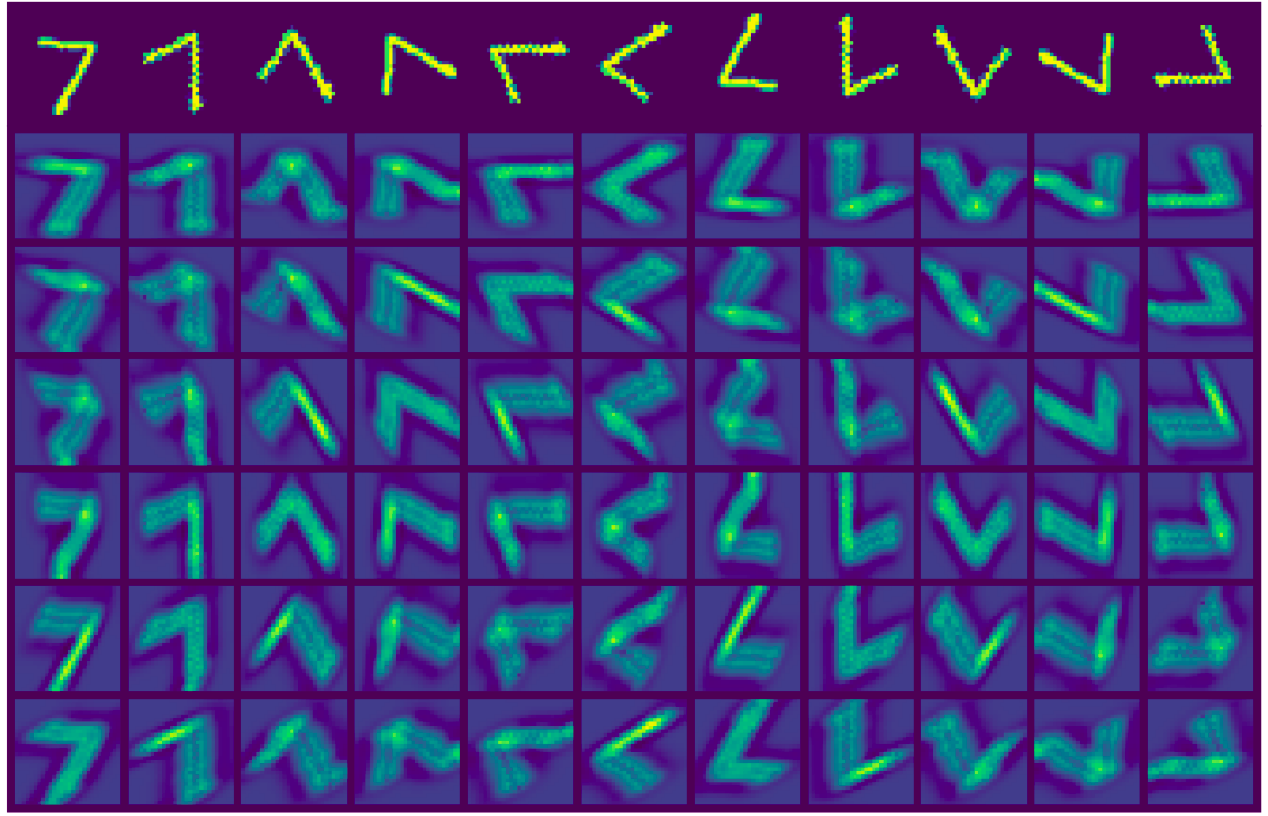
\includegraphics[width=0.6\textwidth]{Images/chebconv_filters.png}
    \caption{Rotation equivariance of a Kaiming initialized $SE(2)$ Chebyshev convolutional layer.}
    \label{fig:7_filters}
\end{figure*}

An efficient implementation of the layer is based on two assumptions. First, assuming the graphs are sparse enough, the graph Laplacian is too. In terms of computation time\footnote{In fact, sparse operations becomes faster than dense ones for very high sparsity rate, typically $0.985$.} and memory consumption, it becomes worth it to use sparse operations instead of dense ones. Second, because the Chebyshev convolutional layer is domain depend, defining convolution in the frequency domain has an inherent drawback of inability to adapt the model across different domains. Thus, we can assume graphs can be defined at the beginning of the algorithm and, up to some small edges and vertices' perturbations, they will not change. Consequently, it is worth it to pre-compute all graphs at the beginning of the algorithm and update each graph Laplacian according to the small perturbations added to the graph instead of computing the graph for each batch.


\subsubsection{Spatial pooling and spatial unpooling layers}

Graph pooling is a central component of a myriad of graph neural network architectures. As an inheritance from traditional CNNs, most approaches formulate graph pooling as a cluster assignment problem, extending local patches' idea in regular grids to graphs. We propose similar operations, based on the spatial domain and involving two steps. First, each sample is assigned to a cluster that will correspond to the output sample  ; this is the down- (resp. up-) sampling phase.\footnote{While down- and up-samplings are pretty obvious on the Euclidean grid, they are not as simple on the sphere. Nevertheless, using an icosahedron decomposition of the sphere makes the task easier as we can just step-down or step-up the subdivision level.} Then each cluster is reduced (resp. expanded) according to a given scheme (e.g. maximum, average or random); this is the reduction (resp. expansion) phase. Producing coarsened graphs from a finer graph have two main advantages: first, it reduces the computational cost, and second, it could improve performance by reducing the overfitting effect. While many algorithms have been proposed for graph pooling \citep{dhillon2007weighted, ying2018hierarchical, khasahmadi2020memory}, it seems that the real influence of pooling procedures on the success of graph neural networks remains to be investigated. The first results of  \cite{mesquita2020rethinking} on this subject are baffling. 

\haguettaz{Figures pooling and unpooling?}

\subsubsection{Random sub-graph}

While a GEChebNet is supposed to be an (almost)-equivariant neural network, an equivariance leakage effect can be observed as the model is specializing on a given task (Appendix \ref{app:equivariance_leakage}). To alleviate this problem, we propose two simple methods, based on a perturbation of the training process as \cite{srivastava2014dropout} did when they introduced dropout. Both method consist on randomly pruning the original graph to construct a random sub-graph. This perturbation can be made once per training epoch or at an higher frequency (per batch or even per sample).

\paragraph{Edges-based random subgraph.} 
A random sub-graph is created by randomly removing edges of the original graph. Based on the weights of the edges, a rate $1 - \kappa_\mathcal{E}$ of edges\footnote{Recently, \cite{keriven2020convergence} studied the convergence of quasi-sparse large random graphs to their continuous counterpart as the number of vertices grows. A direct consequence of their work is that even by randomly sampling the graph's edges, the graph Laplacian still remain consistent.} are discarded. It might be the case that a vertice becomes isolated during the process, meaning that all edges from and to this vertex have disappeared. It is not necessarily a problem, but it is important to be aware of this effect. 
\paragraph{Vertices-based random subgraph.}  
A random sub-graph is created by randomly removing a rate $1-\kappa_\mathcal{V}$ of vertices of the original graph. For the pruning being complete, edges from or to a discarded vertex should also be removed\footnote{Note that since the vertices are uniformly distributed and they all have similar neighborhood (up to boundaries effect) it is equivalent to prune vertices based on their degree.}. This method is more drastic and should be used carefully, as such a vertices pruning leads to a violation of the uniform distribution of vertices that is required for consistency of the graph Laplacian. 

\begin{figure*}[h!] 
    \centering
    \begin{subfigure}[b]{0.48\textwidth}
        \centering
        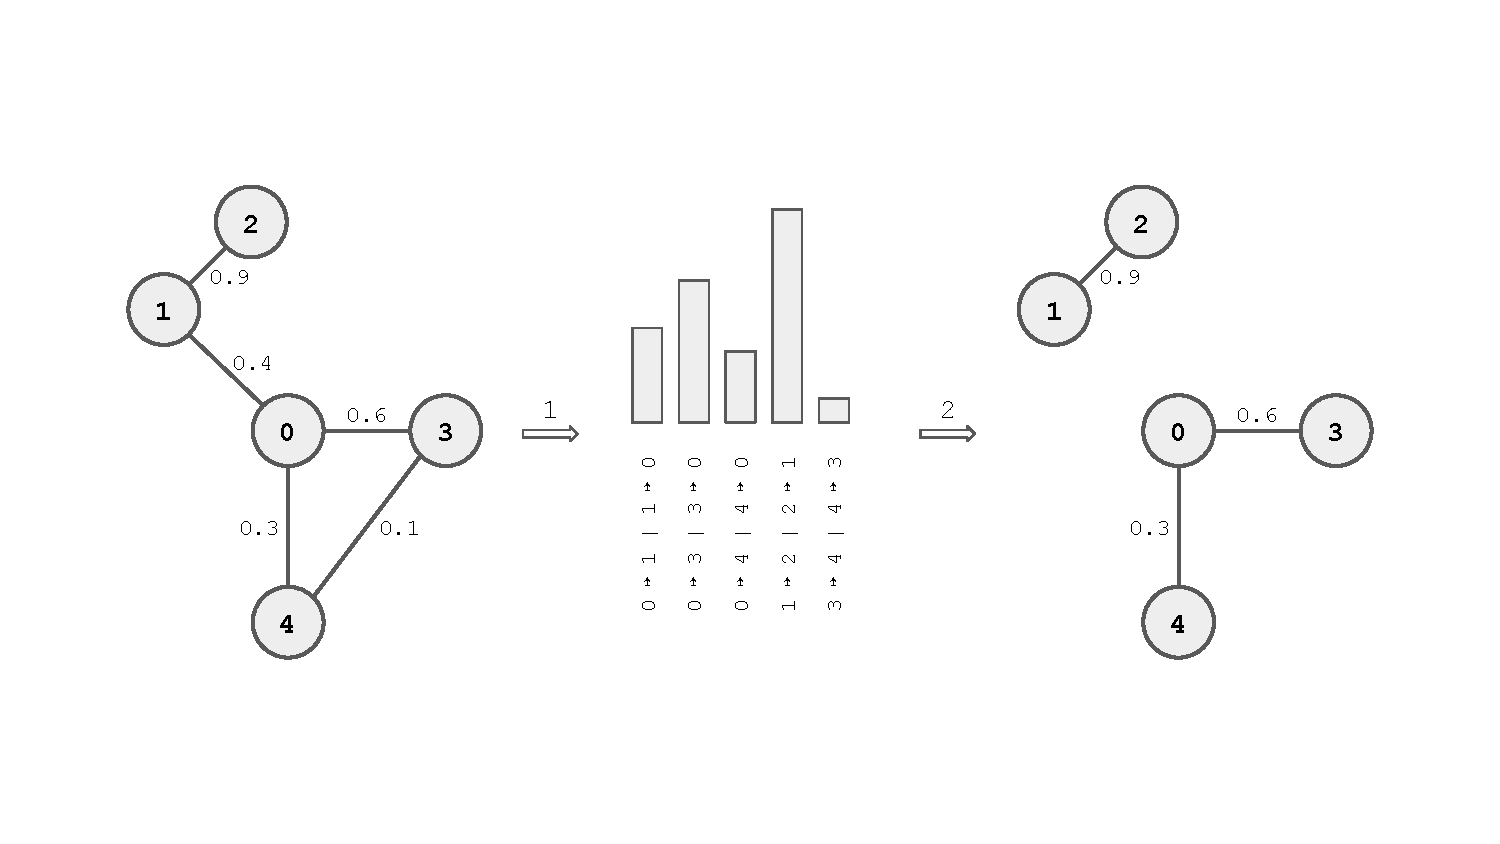
\includegraphics[width=\textwidth]{Images/edge_sampling.pdf}
        \caption{Edges sampling method with $\kappa_\mathcal{E} = 0.6$: 1) a p.m.f. based on the edges' weight is computed 2) $\kappa_\mathcal{E} |\mathcal{E}|$ are sampled according to the p.m.f.}
    \end{subfigure}
    \hfill
    \begin{subfigure}[b]{0.48\textwidth}
        \centering
        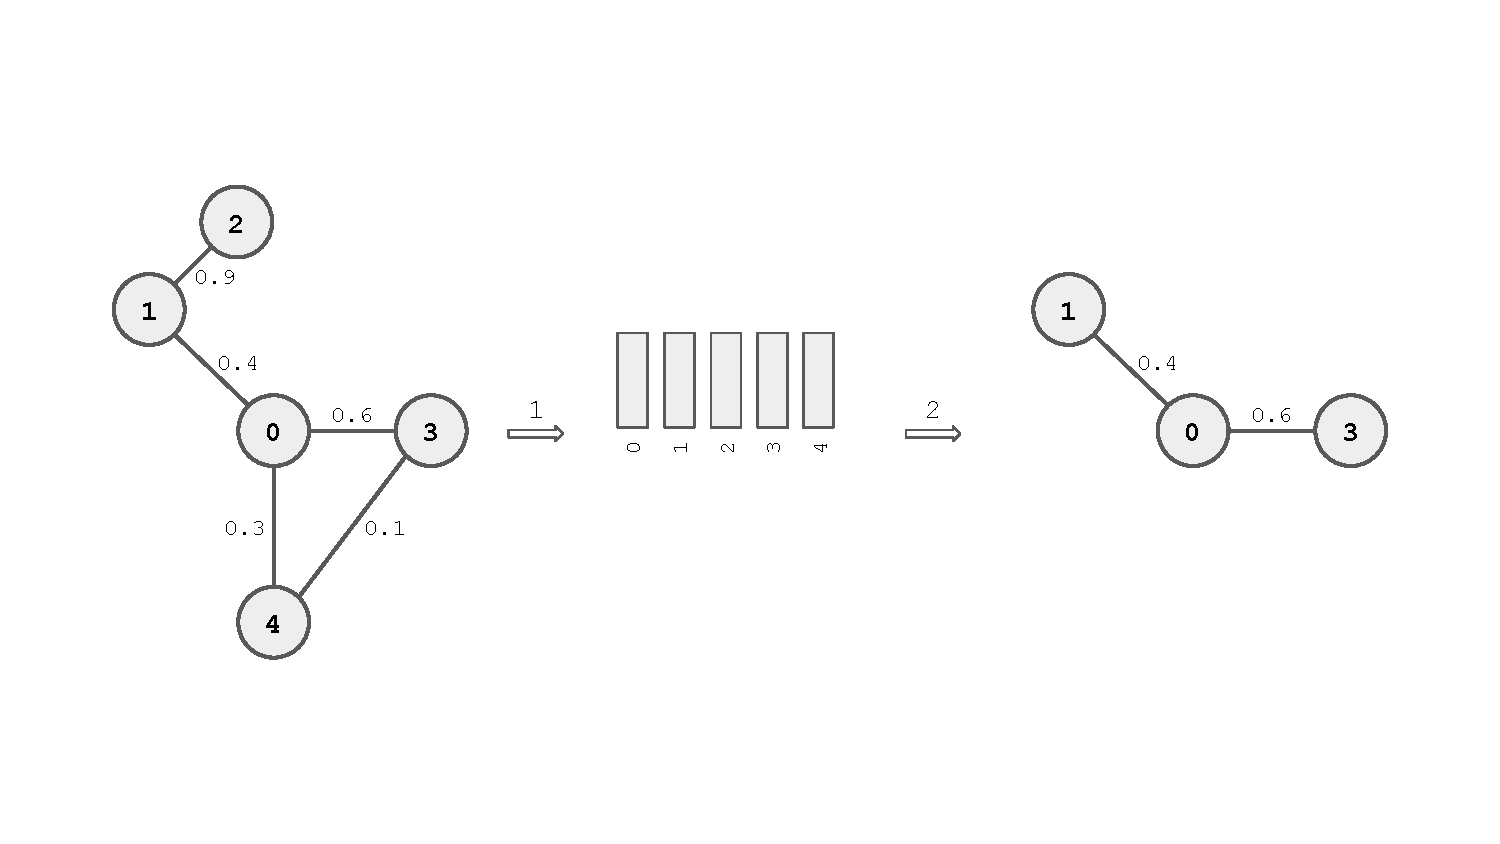
\includegraphics[width=\textwidth]{Images/vertex_sampling.pdf}
        \caption{Vertices sampling method with $\kappa_\mathcal{V} = 0.6$: 1) a uniform p.m.f. over the vertices is computed 2) $\kappa_\mathcal{V} |\mathcal{V}|$ are sampled according to the p.m.f.}
    \end{subfigure}
    \caption{Edges and vertices sampling methods.}
    \label{fig:sampling}
\end{figure*}

\section{Experiments} \label{sec:experiments}

To demonstrate the good potential of our method, we perform experiments with the groups $SE(2)$ and $SO(3)$, and evaluate the effect of using anisotropic filters instead of isotropic ones. Even if the spatial anisotropy is quite modulable, we will focus on extreme spatial anisotropies ($\varepsilon = 0.1$). In future research, it could be interesting to evaluate moderate spatial anisotropies (e.g., $0.3 \leq \varepsilon \leq 0.5$). For each experiment, we use 8 nearest neighbors graphs and adapt the orientation anisotropy parameter to reach a ratio 40/60 on 6 orientation layers.\footnote{It means each vertex has around 40\% of its neighbors on the same orientation layer and 60\% on other layers.} 

While we are trying to build competitive networks, the experiments aims not to reach state-of-the-art performance as they require hyper-parameters optimization \citep{yu2020hyper}. All ChebNet-like neural networks are deep, meaning that we should use different tools to help going deeper (residual convolutional layers \citep{he2016deep}, batch normalization \citep{ioffe2015batch}, rectified linear units \citep{nair2010rectified}, ADAM optimizer \citep{kingma2014adam},  Kaiming initialization \citep{he2015delving}) with resized batches to fit the available CUDA memory. Our implementation is fully PyTorch \citep{pytorch} and available at \url{https://github.com/ebekkers/GroupEquivariantChebNets}. We performed all the experiments on a single GeForce GTX 1080 Ti GPU and tracked them with Weights \& Biases \citep{wandb}. 

\subsection{Projective line bundle of the $SE(2)$ group}

In this bunch of experiments, we evaluate wide residual architectures \citep{zagoruyko2016wide} on CIFAR10 \citep{krizhevsky2009learning} and STL10 \citep{coates2011analysis}, for image classification tasks. We used 2 random spatial pooling layers as they get similar performance than maximum and average spatial pooling but seems to slightly reduce over-fitting. We set $\xi \in \{0.0019, 0.008, 0.032\}$ (resp. $\xi \in \{0.0002, 0.0009, 0.0036\}$) for CIFAR10 (resp. STL10) and use a 2-deep 4-wide (3-deep 4-wide) neural network with convolution kernel of size 4 (resp. 3), leading to a neural network with $\sim \SI{315}{\kilo\nothing}$ (resp. $\sim \SI{1.2}{\mega\nothing}$) trainable parameters for CIFAR10 (resp. STL10).

\begin{table}[h!]
\centering 
\caption{Mean of test accuracies and training duration on CIFAR10 and STL10. Errorbars are 1 standard deviation computed over 5 trials.}
\begin{tabular}{c c c c c}
\toprule
 & \multicolumn{2}{c}{CIFAR10} & \multicolumn{2}{c}{STL10} \\
$\varepsilon$ & Test accuracy & Duration & Test accuracy & Duration \\
\midrule
$1$ & $77.43 \pm 0.31 \%$ & $\sim \SI{5}{\hour}$ & $68.98 \pm 0.56 \%$ & $\sim \SI{9}{\hour}$ \\
$0.1$ & $\boldsymbol{83.94 \pm 0.10 \%}$ & $\sim \SI{8}{\hour}$ & $\boldsymbol{74.02 \pm 1.10 \%}$ & $\sim \SI{16}{\hour}$ \\
\bottomrule
\end{tabular}
\end{table}

\subsection{Projective line bundle of the $SO(3)$ group}

To evaluate our method on spherical data, we choose a segmentation task on the meteorological dataset ClimateNet \citep{kashinath2021climatenet}. The objective is to detect extreme meteorological events (atmospheric rivers and tropical cyclones) at the surface of the Earth, based on 16 pointwise informations. We use a U-Net-like architecture \citep{ronneberger2015u} with 6 levels and spatial maximum pooling (encoding) and spatial average unpooling (decoding). We set $\xi \in \{0.001, 0.004, 0.0156, 0.0617, 0.2381, 0.8333\}$ (ascending order of graph finesse) and use convolutional kernel of size 4, leading to around $\SI{1.2}{\mega \nothing}$ trainable parameters. 

\begin{table}[h!]
\centering 
\caption{Mean of test accuracies and training duration on ClimateNet. Errorbars are 1 standard deviation computed over 3 trials.}
\begin{tabular}{c c c c c c c}
\toprule
 & \multicolumn{6}{c}{ClimateNet} \\
$\varepsilon$ & Test BG & Test AR & Test TC & Test mAP & Test F1 & Duration \\
\midrule
$1$ & $99.78 \pm 0.27 \%$ & $56.98 \pm 1.78 \%$ & $92.45 \pm 1.29 \%$ & $74.63 \pm 0.25 \%$ & $\boldsymbol{85.62 \pm 0.09 \%}$ & $\sim \SI{2}{\day}$ \\
$0.1$ & & & & & $85.25 \pm 0.19 \%$ & $\sim \SI{7}{\day}$ \\
\bottomrule
\end{tabular}
\end{table}

These experiments do not aim to demonstrate the state of the art's performances but only show that we have something to benefit from anisotropic kernels. While the anisotropic GEChebNet is slower to train than the isotropic one, the accuracy's improvement is significant for the SE(2) group, as the extreme anisotropic kernels outperform the isotropic ones by more than $5\%$ test-accuracy on CIFAR10 and STL10. We do not show results on MNIST here since it is not challenging enough, according to us. The difference in accuracy is less significant, as both models saturated at most than $99\%$ accuracy on the test set. For the SO(3) group, the use of extreme anisotropic kernels is neither beneficial nor detrimental in terms of the models' performance. Nevertheless, these experiments show one important thing: the anisotropies requirements are data-dependent, therefore the anisotropies-controllable feature of our approach is a crucial asset and the main strength of the GEChebNets.

\haguettaz{comment so3 performance + add something about mAP and per class accuracy}

\section{Scope, limitations and future research} \label{sec:scope_limitations_future_research}

\paragraph{Scope.} As it is able to model any Lie group, our method is extendable to many datasets. Using $SE(2)$ group, we can get a roto-translation equivariant neural network for $2D$ images or videos. With the higher dimensional group $SE(3)$, the method can solve a task involving 3-dimensional shapes requiring roto-translation equivariance. On the sphere and using the group $SO(3)$, the method can deal with meteorological or cosmological data while preserving rotation equivariance. For each task, it is necessary to exist an orientation axis, based on which we can steer the anisotropic kernels.

\paragraph{Limitations.} The main weakness of our method is its high memory requirements. By adding an orientation axis, we significantly enlarge the feature maps. As a result, anisotropic graph manifolds are memory-heavier than isotropic ones and prone to overfitting and slowdown during forward and backward pass. Nevertheless, with the emergence of graph-based machine learning algorithms, we expect cutting-edge technologies to become more performant on graph data. We hope the advances in quantum machine learning will help alleviate this problem in the next few years. At the present moment, it is still possible to use some dedicated libraries such as PyKeops \citep{charlier2020kernel}. This memory-efficient library relies on the concept of symbolic matrices and takes advantage of CUDA registers' structure to bypass costly memory transfers and achieve optimal runtimes on a wide range of applications. Another difficulty of our method is its high number of hyper-parameters on which we only have some rule of thumb to set them. The graph connectivity requires a tradeoff between efficiency and quality of the group approximation. The anisotropic parameters require a deep analysis of the dataset and some intuition about the necessity of using anisotropic kernels and how strong we should set these anisotropies. The similarity kernel bandwidth is also hard to set. With a systematic hyper-parameter optimization \citep{yu2020hyper}, we can find an optimal combination, but it requires many computational resources.


\paragraph{Future research.} As it has been mentioned earlier, it could be interesting to launch a deep ablation study about the model's hyper-parameters (orientation resolution, anisotropies, graph connectivity, etc.). In particular, some questions remain. Do we need to use an higher graph connectivity for an anisotropic GEChebNet than for an isotropic one, as the neighborhood of a vertex is spread over several orientation layers? How to easily set intensities of the spatial anisotropies, could we use an heuristic for that? How strong should be the connection between orientation layers? 

\haguettaz{convergence of graph laplacian to anisotropic Laplace Beltrami operator?}



\section{Conclusion} \label{sec:conclusion}

In this paper, we studied the premises of a novel deep learning approach. We introduced the anisotropic manifold graph, an abstract object whose purpose is to approximate a transformation group. Using such objects when constructing neural networks, we developed Group Equivariant ChebNets (GEChebNets) with anisotropic kernels. Group equivariance is achieved via anisotropic spectral (Chebyshev) graph convolutions on graphs with anisotropic left-invariant Riemannian distance-based affinities encoded on the edges. The strength of our approach is its complete control over anisotropy parameters. Through experiments on CIFAR10, STL10, and ClimateNet, we showed that our method deserves further analysis, as it gives promising results and a first overview of the benefits we can get from using anisotropic kernels instead of isotropic ones.


\begin{ack}
Thanks to ...
\end{ack}

\clearpage
\bibliographystyle{plainnat}
\bibliography{bibliography}

%%%%%%%%%%%%%%%%%%%%%%%%%%%%%%%%%%%%%%%%%%%%%%%%%%%%%%%%%%%%
\clearpage
\section*{Checklist}

%%% BEGIN INSTRUCTIONS %%%
The checklist follows the references.  Please
read the checklist guidelines carefully for information on how to answer these
questions.  For each question, change the default \answerTODO{} to \answerYes{},
\answerNo{}, or \answerNA{}.  You are strongly encouraged to include a {\bf
justification to your answer}, either by referencing the appropriate section of
your paper or providing a brief inline description.  For example:
\begin{itemize}
  \item Did you include the license to the code and datasets? \answerYes{See Section~\ref{gen_inst}.}
  \item Did you include the license to the code and datasets? \answerNo{The code and the data are proprietary.}
  \item Did you include the license to the code and datasets? \answerNA{}
\end{itemize}
Please do not modify the questions and only use the provided macros for your
answers.  Note that the Checklist section does not count towards the page
limit.  In your paper, please delete this instructions block and only keep the
Checklist section heading above along with the questions/answers below.
%%% END INSTRUCTIONS %%%

\begin{enumerate}

\item For all authors...
\begin{enumerate}
  \item Do the main claims made in the abstract and introduction accurately reflect the paper's contributions and scope?
    \answerYes{See Section~\ref{sec:introduction}}
  \item Did you describe the limitations of your work?
    \answerYes{See Section~\ref{sec:conclusion}}
  \item Did you discuss any potential negative societal impacts of your work?
    \answerTODO{}
  \item Have you read the ethics review guidelines and ensured that your paper conforms to them?
    \answerTODO{}
\end{enumerate}

\item If you are including theoretical results...
\begin{enumerate}
  \item Did you state the full set of assumptions of all theoretical results?
    \answerYes{See Section~\ref{sec:method}}
	\item Did you include complete proofs of all theoretical results?
    \answerYes{We refer the reader to original publication with proofs.}
\end{enumerate}

\item If you ran experiments...
\begin{enumerate}
  \item Did you include the code, data, and instructions needed to reproduce the main experimental results (either in the supplemental material or as a URL)?
    \answerYes{See Section~\ref{sec:method}}
  \item Did you specify all the training details (e.g., data splits, hyperparameters, how they were chosen)?
    \answerYes{See Section~\ref{sec:experiments}}
	\item Did you report error bars (e.g., with respect to the random seed after running experiments multiple times)?
    \answerYes{See Section~\ref{sec:experiments}}
	\item Did you include the total amount of compute and the type of resources used (e.g., type of GPUs, internal cluster, or cloud provider)?
    \answerYes{See Section~\ref{sec:experiments}}
\end{enumerate}

\item If you are using existing assets (e.g., code, data, models) or curating/releasing new assets...
\begin{enumerate}
  \item If your work uses existing assets, did you cite the creators?
    \answerYes{See Section~\ref{sec:experiments}}
  \item Did you mention the license of the assets?
    \answerNA{}
  \item Did you include any new assets either in the supplemental material or as a URL?
    \answerNA{}
  \item Did you discuss whether and how consent was obtained from people whose data you're using/curating?
    \answerNA{}
  \item Did you discuss whether the data you are using/curating contains personally identifiable information or offensive content?
    \answerNA{}
\end{enumerate}

\item If you used crowdsourcing or conducted research with human subjects...
\begin{enumerate}
  \item Did you include the full text of instructions given to participants and screenshots, if applicable?
    \answerNA{}
  \item Did you describe any potential participant risks, with links to Institutional Review Board (IRB) approvals, if applicable?
    \answerNA{}
  \item Did you include the estimated hourly wage paid to participants and the total amount spent on participant compensation?
    \answerNA{}
\end{enumerate}

\end{enumerate}

%%%%%%%%%%%%%%%%%%%%%%%%%%%%%%%%%%%%%%%%%%%%%%%%%%%%%%%%%%%%

\appendix

\section{Background} \label{sec:background}

\subsection{Riemannian geometry}

Riemannian geometry is a part of differential geometry that studies Riemannian manifolds, smooth manifolds equipped with a Riemannian metric. A manifold $\mathcal{M}$ is a generalization and abstraction of the notion of a curved surface. It is a topological set that is modeled closely on Euclidean space locally but may vary widely in global properties. It means for each $p \in \mathcal{M}$, we can associate a tangent space $T_p(\mathcal{M}) \subseteq \mathbb{R}^d$, corresponding to the union of all tangent vectors of differentiable curves passing through $p$. Consequently, at any point $p \in \mathcal{M}$, the tangent space $T_p(\mathcal{M})$ is spanned by a basis $\{\partial_{x_i, p} \}_{i=1}^N$:
\begin{equation}
T_p(\mathcal{M}) = \{ \dot{\gamma}(0) | \gamma : \mathbb{R} \to \mathcal{M} \in \mathcal{C}^1 \text{and } \gamma(0) = p\} = \spn\{\partial_{x_i,p} \}_{i=1}^N.
\end{equation}
A Riemannian manifold is a differentiable manifold $\mathcal{M}$ with a Riemannian metric $\mathcal{R}$, a 2-tensor field, such that at each $p \in \mathcal{M}$, we have a function $\mathcal{R}|_p : T_p (\mathcal{M}) \times T_p(\mathcal{M}) \to \mathbb{R}$ which is symmetric and positive definite. At each $g \in G$, the Riemannian metric can be expressed by its local representation, a symmetric positive definite matrix $\boldsymbol{R}_p$ whose components are given by:
\begin{equation}
r_{ij}(p) = \mathcal{R}|_p (\partial_{x_i, p}, \partial_{x_j, p}).
\end{equation}
In the following we consider Riemannian metric with  diagonal local representation at the origin $e$, that is:
\begin{equation}
r_{ij}(e) = \left\{
    \begin{array}{ll}
        r_{i} & \text{if } i = j  \\
        0 & \text{otherwise}
    \end{array}
\right..
\end{equation}
The Riemannian metric induces an inner product, such that for any $u = u^i \partial_{x_i, e}$ and $v = v^i \partial_{x_i, e}$, we have $\langle u, v \rangle_{\mathcal{R}(e)} = u^i r_i v^i$ and $|| u ||_{\mathcal{R}(e)}^2 = u^i r_i u^i$. Between each pair of points $p$ and $q$ of a Riemannian manifold, we define their Riemannian distance as the length of the shortest curve connecting the two points (a.k.a. geodesic). More formally, we have:
\begin{equation}
d(p, q) = \inf_{\gamma \in \mathcal{C}^\infty_{p, q}} \int_0^1 ||\dot{\gamma}(\tau)||_{\mathcal{R}_{\gamma(\tau)}} d\tau,
\end{equation}
where $\mathcal{C}^\infty_{p, q} = \{ \gamma : [0, 1] \to \mathcal{M} | \gamma \in \mathcal{C}^\infty, \gamma(0) = p,  \gamma(1) = q\}$. An more convenient way to define the Riemannian between two points is via the exponential and logarithmic Riemannian maps (Figure \ref{fig:explogmap}). The Riemannian exponential map $\exp_p T_p(\mathcal{M}) \to \mathcal{M}$ is defined as:
\begin{equation}
\exp_p (v) = \gamma_{p, v}(1) ,\qquad (\text{and by extension } \exp_p (tv) = \gamma_{p, v}(t)),
\end{equation}
where $\gamma_{p,v}(1)$ is the unique Riemannian geodesic starting at $p \in \mathcal{M}$ with initial velocity $v \in T_p(\mathcal{M})$. We can interpret the exponential map as follows. Let’s choose any direction in our tangent space and follow it with a step forward. We make sure to take the shortest path and end up at a new point. This process is what we called the exponential map.\footnote{It comes from the fact that all these tiny steps magically resemble the series expansion of the exponential function.} The inverse mapping of the exponential map, the logarithmic map $\log_p : \mathcal{M} \to T_p(\mathcal{M})$ will map an element $p \in \mathcal{M}$ to the smallest vector $v = \log_p q \in T_p(\mathcal{M})$ as measured by the Riemannian metric such that $q = \exp_p v \in \mathcal{M}$. 

\begin{figure*}[h!]
    \centering
    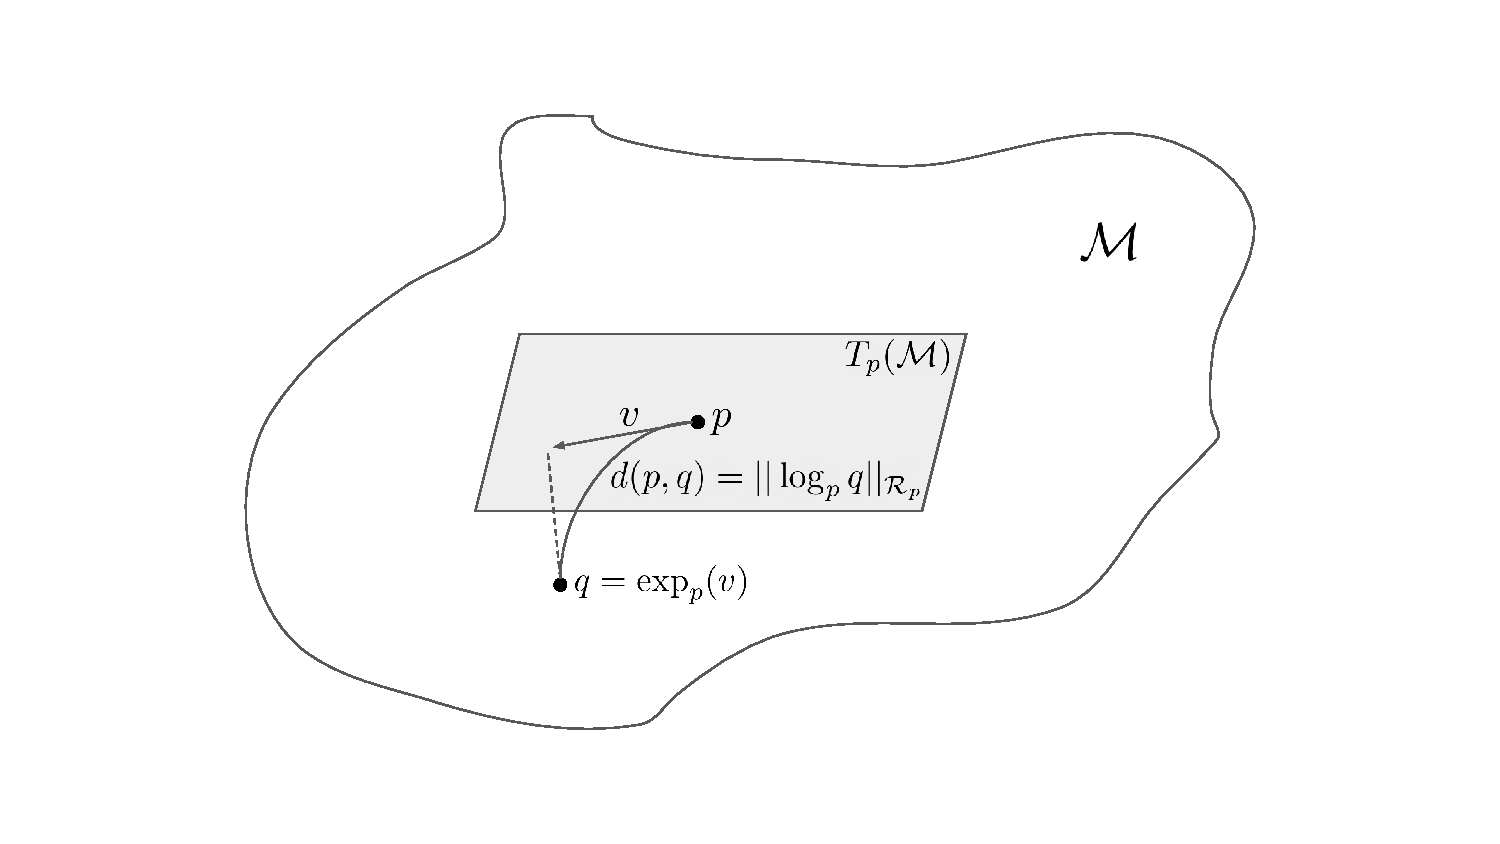
\includegraphics[width=\textwidth]{Images/distexplog.pdf}
    \caption{Riemannian exponential map $\exp_p : T_p(\mathcal{M}) \to \mathcal{M}$ and Riemannian logarithmic map $\log_p : \mathcal{M} \to T_p(\mathcal{M})$.}
    \label{fig:explogmap}
\end{figure*}


\subsection{Group theory}

A rigorous investigation of an operator property of equivariance under a group transformation, require a bit of knowledge in group theory. A group $(G, \cdot)$ is a set $G$ equipped with a binary operation $\cdot : G \to G$ called group product, satisfying the four group axioms (closure, associativity, identity element and inverse elements). To map the structure of the group to some mathematical object, one requires a representation. We define $H$ as the vector space to which our mathematical object belongs and $\mathcal{B}(H)$ the space of bounded linear invertible operators $H \to H$. A representation $\mathcal{V} : G \to \mathcal{B}(H)$ maps a group element to an operator such that the identity element, the group product and the group inverse are preserved. We define the left-regular representation $\mathcal{L}_g$ on the (infinite-dimensional) vector space of functions $G \to \mathbb{R}^d$ via:
\begin{equation}
(\mathcal{L}_g \circ f )(h) = f(g^{-1}h),
\end{equation}
with $f : G \to \mathbb{R}^d$ a function on the group $G$ and $g, h$ elements of the group $G$. Using this group representation, we can formally define the left-invariance (a.k.a. equivariance).

\begin{definition}[Equivariance] \label{def:equivariance}
An operator $\Phi : \mathcal{X} \to \mathcal{Y}$ from one vector space to the other is equivariant (or left-invariant under group transformation) if it satisfies the following property:
\begin{equation}
\mathcal{L}'_g \circ \Phi = \Phi \circ \mathcal{L}_g, \qquad \forall g \in G.
\end{equation}
\end{definition}

Equivariance can be realized in many ways, and in particular, the group representations $\mathcal{L}_g$ and $\mathcal{L}'_g$ need not be the same, as they act on different spaces $\mathcal{X}$ and $\mathcal{Y}$. Note that the familiar concept of invariance is a special kind of equivariance where  $\mathcal{L}_g'$ is the identity transformation for all element $g$ of the group $G$. We define the equivariance error, a measure of the equivariance of an operator.

\begin{definition}[Equivariance error] \label{def:equiv_err}
Let $\Phi : \mathbb{L}_2(G) \to \mathbb{L}_2(G)$ be an operator and $g$ an element of a group $G$ with left regular representation $\mathcal{L}_g$. The equivariance error of the operator $\Phi$ is given by:
\begin{equation}
\varepsilon(g, f) = \frac{|| (\mathcal{L}'_g \circ \Phi )(f) - ( \Phi \circ \mathcal{L}_g) (f)||_2^2}{|| (\mathcal{L}'_g \circ \Phi )(f)||_2^2}, \qquad f \in \mathbb{L}_2(G).
\end{equation}
\end{definition}

A Lie group is a continuous group whose group elements are parameterized by a finite-dimensional differentiable manifold. In essence, this means that a Lie group is a group to which we can apply differential geometry. From now on, we also assume the group manifold is equipped with a Riemannian metric, that is it is Riemannian manifold. To each element $g$ of $G$, we can associate a tangent space $T_g(G)$, which is spanned by a basis of left-invariant vectors denoted by $\{\mathcal{A}_i|_g\}_{i=1}^n$. We write $T_g(G) = \spn\{\mathcal{A}_1|_g, \dots, \mathcal{A}_n|_g\}$ and we can express tangent vectors $\dot{\gamma}(t)$ of $T_g(G)$ in this basis via $\dot{\gamma}(t) = c^i(t) \mathcal{A}_i|_{\gamma(t)}$.

Moreover, because this frame of basis vector is left-invariant, the coefficients $c_i(t)$ remain unchanged if the curve is moved by applying left group product. The tangent space at the origin $T_e(G)$ is spanned by a basis $\{A_i\}_{i=1}^n$ where $A_i = \mathcal{A}_i|_e$. We make a subtle difference in notation between $\mathcal{A}$ and $A$, where $\mathcal{A}$ represents a whole vector field and $\mathcal{A}|_g$ represents the vector at location $g$. The straight $A$ is used to indicate a vector in the Lie algebra, the tangent space at the origin. Via the push-forward $(L_g)_*$, we can generate a whole vector space by picking a vector in the Lie algebra and transporting tangent vectors from $\dot{\gamma}(0) \in T_e(G)$ to $g \cdot \dot{\gamma}(0) \in T_g(G)$ using:
\begin{equation}
\mathcal{A}_i|_g = (L_g)_* A_i , \qquad \forall g \in G.
\end{equation}

The left-invariant frame of basis vectors could also be interpreted as the directional derivative of functions defined on the group $G$. At any element $g$, the value of the directional derivative of a function $f$ defined on $G$ can be computed using the push-forward operation:
\begin{equation}
\mathcal{A}_i|_g f = (L_g)_* \mathcal{A}_i|_e f := \mathcal{A}_i|_e (f \circ L_{g^{-1}}),
\end{equation}
so $\mathcal{A}_i|g f$ represents the directional derivative along the vector field at location $g$, which can be defined by translating the function back to the origin via $L_{g^{-1}}$ and compute the derivative at the origin along the direction specified by $\mathcal{A}_i|_e$. In the above $L_g h:= g h$.
 
The Laplace-Beltrami operator, the generalization to Riemannian manifold of the Laplace operator\footnote{Another equivalent definition in local coordinates exists too. It explicitly takes into account the Riemannian metric tensor field $\mathcal{R}$ previously defined. Here we use a more compact definition but using the subscript $\mathcal{R}(g)$ to indicate that the Laplace-Beltrami operator depends on the location on the Riemannian manifold and the Riemannian metric tensor field.} is defined below. 
\begin{definition}[Laplace-Beltrami operator] \label{def:laplace_beltrami}
Let $g$ be an element of the Lie group $(\mathcal{M}, \cdot)$. The Laplace-Beltrami operator on the Riemannian manifold $\mathcal{M}$ is defined as 
\begin{equation}
\Delta_{\mathcal{R}(g)} = \dive (\nabla_{\mathcal{R}(g)})
\end{equation}
\end{definition}

Using the left-invariant frame of basis vectors as directional differential operators, we can define the gradient, expressed as a vector relative to the basis $\mathcal{A}_i|_g$, of a function $f : G \to G$:
\begin{equation}
\nabla_{\mathcal{R}(g)} f = \mathbf{R}_{g}^{-1} (\mathcal{A}_1|_g f, \dots, \mathcal{A}_n|_g f)^\top,
\end{equation}
where $\mathbf{R}_{g}$ is the Riemannian metric tensor defined relative to the basis $\mathcal{A}_i$, that corrects for local scaling and shrinking of the manifold as measured by the metric tensor.
The divergence of a vector field $F : G \to \mathbb{R}^n$ is the operator:
\begin{equation}
\dive(F) = \sum_{i=1}^n \mathcal{A}_i|_g F_i.
\end{equation}

The Laplace-Beltrami operator depends on a Riemannian metric tensor, which describes how lengths of vectors should be measured in different directions, and in the Laplace-Beltrami operator, it rescales the derivates accordingly. While the usual Laplacian is isotropic (derivatives are threated the same in each direction), the Laplace-Beltrami operator can be anisotropic due to the Riemannian metric that is used.

\begin{theorem}[Left-invariance of the Laplace-Beltrami operator] \label{thm:equiv_laplace_beltrami}
The Laplace-Beltrami operator $\Delta_{\mathcal{R}(g)}$ is left-invariant and satisfies:
\begin{equation}
\Delta_{\mathcal{R}(g)} = (L_g)_* \Delta_{\mathcal{R}(e)}.
\end{equation}
\end{theorem}


A Lie algebra $\mathfrak{g}$ is a vector space (here the tangent space at the identity element $T_e(G)$) that is endowed with a binary operator called the Lie bracket or commutator $[\cdot, \cdot] : T_e(G) \times T_e(G) \to T_e(G)$ that is bilinear, alternative and satisfies the Jacobi identity. Conceptually, the Lie bracket $[A, B]$ of two vector fields $A, B$ is the derivative of $B$ along the flow generated by $A$.\footnote{Two vector fields are commutative (zero Lie bracket) if and only if its flows are too, in the sense that there is no difference starting at one point $p$, traveling a time $t_a$ over the flow of $A$ and then a time $t_b$ over the flow of $B$, or, instead, traveling first $t_b$ over the flow of $B$ and then $t_a$ over the flow of $A$.} In the following, we take $\{A_i\}_{i=1}^n$ with $A_i = \mathcal{A}_i|_e$ as Lie Algebra and get left-invariant vector fields via the push-forward operation. 

The Lie group exponential and logarithmic maps define the mappings between the group and the tangent space. The exponential map on a Lie group can be thought of as picking a vector $A$ in the Lie algebra, construct a left-invariant vector field $\mathcal{A}$ via the push-forward operator, and follow this vector field by taking infinitesimal steps along the direction indicated by the vector field. Integrating along the vector field defined by $A$ for unit time brings to some point $g \in G$. So $g = \exp A$, where $\exp: \mathfrak{g} \to G$.\footnote{Note that Riemannian and Lie group exponential maps are different. For the general Riemannian exponential map, the vector field along which we compute the path integral is defined by the Riemannian metric. In the Lie group exponential map, the vector field is defined by the push forward of left-multiplication. The curves defined by the path integrals in the Riemannian exponential are known to be geodesics. The exponential curves in the Lie group case are "straight curves" with respect to a moving frame of reference but are not necessarily geodesics. The Riemannian and Lie group exponential maps only coincide when the Riemannian metric is both left and right invariant (see Section 4.5 in \citet{bekkers2017thesis}).}



\subsection{Graph theory}

Graphs are generic data representation forms that are useful for describing the geometric structure of data domains \citep{west1996introduction}. More formally, we define a graph $\mathcal{G}$ as a structure modeling a finite set of interactions called edges $\mathcal{E}$ between a finite set of objects called vertices $\mathcal{V}$. In the following, we denote by $|\mathcal{V}|$ the size of the set of vertices, that is, the number of vertices in the graph, and by $|\mathcal{E}|$ the size of the set of edges, that is the number of edges in the graph. We denote $v_i$ the $i$-th vertex and $e(v_i, v_j)$ the potential edge from $v_i$ to $v_j$. We call the neighborhood of the vertex $v_i$ the set of vertices connected to $v_i$ by an edge and denote it by $\mathcal{N}(v_i)$. More generally, we write $\mathcal{N}^k(v_i)$ for the $k$-hops neighborhood of vertex $v_i$, that is, the set of vertices connected to $v_i$ with a path of at most $k$ edges. In some cases, it can be useful to add weights on graph edges. In general, the weights can take any value. Nevertheless, in this thesis, we assume weights in the range $[0, 1)$ and measuring the similarity rather than the distance. When the edges' weights\footnote{The terms similarity kernel and similarity measure are interchangeable terms for weight kernel and edge's weight.} are not naturally defined by an application, a common way to define them is to apply a kernel $\mathfrak{K} : \mathbb{R}_+ \to [0, 1)$ on the distance between connected nodes. For theoretical convergence results, we will use a Gaussian weighting scheme in the following: 
\begin{equation}
w(v_i, v_j) =
\left\{ 
\begin{array}{ll}
\exp \left(- \frac{d^2(v_i, v_j)}{4t}\right) & \text{if } e(v_i, v_j) \in \mathcal{E} \\
0 & \text{otherwise}
\end{array}
\right.,
\end{equation}
where $d(v_i, v_j)$ denotes the (Riemannian) distance between vertices $v_i$ and $v_j$ and $t$ is a positive real number called bandwidth of the Gaussian kernel. From now on, we furthermore assume that the graphs are undirected and without self-loop.

The field of signal processing on graphs merges algebraic and spectral graph theoretic concepts with computational harmonic analysis to process such signals on graphs \citep{shuman2013gsp}. A signal on a graph is a function $f : \mathcal{V} \to \mathbb{R}^d$, mapping each vertex of the graph to a $d$-dimensional real valued vector. In matrix form, this signal is a $|\mathcal{V}| \times d$ real valued matrix $\boldsymbol{f}$ whose rows are given by $\boldsymbol{f}_i = f(v_i) \in \mathbb{R}^d$. 

An essential object in graph signal processing is the Laplacian operator. Under some specific conditions that we will state later, it can be interpreted as a discrete version of the Laplace-Beltrami operator.
\begin{definition}[Symmetric normalized Laplacian] \label{def:graph_laplacian}
Let $\mathcal{G}$ be an undirected weighted graph without self-loops. The symmetric normalized Laplacian $\boldsymbol{\hat{\Delta}}$ is the $|\mathcal{V}| \times |\mathcal{V}|$ real valued matrix whose components are given by:
\begin{equation}
\hat{\Delta}_{i, j} =
\left\{
\begin{array}{ll}
1 & \text{if } i = j \text{ and } \deg(v_i) > 0 \\
- \frac{w(v_i, v_j)}{\sqrt{\deg (v_i) \deg (v_j)}} & \text{if } i \neq j \text{ and } \deg(v_i) > 0 \\ 
0 & \text{otherwise}
\end{array}
\right..
\end{equation}
\end{definition}

Assuming a function $f$ defined on the graph vertices $\mathcal{V}$, by inspection on the components of $\boldsymbol{\hat{\Delta}}^k \boldsymbol{f}$, we remark that the Laplacian acts as a $k$-op neighborhood operator. We can prove that $\boldsymbol{\hat{\Delta}}$ is a symmetric positive definite matrix. Hence it admits a unique eigendecomposition of the form $\boldsymbol{\hat{\Delta}} = \boldsymbol{\Phi \Lambda \Phi}^\top$ where the $j$-th column of $\Phi$ correponds to the eigenvector $\phi_j$ associated with real positive eigenvalue $\lambda_j$. In these settings, the eigenvalues are in the range $[0, 2]$ \citep{chung1997spectral}. By analogy with the Euclidean case where the Laplacian's eigenfunctions correspond to the Fourier basis, we can construct a graph Fourier basis from the eigendecomposition of the graph Laplacian, and define the graph Fourier transform and its inverse.\footnote{The existence of an inverse transform is a consequence of the orthonormal property of the eigendecomposition}
\begin{definition}[Graph Fourier transform]
Let $\mathcal{G} = (\mathcal{V}, \mathcal{E})$ be a graph with Laplacian $\boldsymbol{\hat{\Delta}}$ and let $f : \mathcal{V} \to \mathbb{R}$ be a signal defined on the graph's vertices. The graph Fourier transform $\hat{f}$ of $f$ is given by:
\begin{equation}
\hat{f}(\lambda_j) = \hat{f}_j = \{ \boldsymbol{\Phi}^\top \boldsymbol{f}\}_j = \sum_i \phi_{ij} f_i = \sum_{v_i} \phi(v_i, \lambda_j) f(v_i),
\end{equation}
and its inverse transform by:
\begin{equation}
f(v_i) = f_i = \{\boldsymbol{\Phi}  \boldsymbol{\hat{f}} \}_i = \sum_j \phi_{ij} \hat{f}_j = \sum_{\lambda_j} \phi(v_i, \lambda_j) \hat{f}(\lambda_j).
\end{equation}
\end{definition}

\clearpage

\section{Lie groups} \label{sec:lie_groups}

At the moment, all the group's elements we are interested in are in 1-1 correspondence with elements of the 3-dimensional general linear group $GL(3)$, the group of $3 \times 3$ real matrices. We will use this representation since working with matrices is more convenient in general. Moreover the Lie group exponential and logarithm coincide with the matrix exponential and logarithm.

For the roto-translation group  $SE(2)$, the spatial part corresponds to the planar translations and the orientation part to the rotation angles. Group elements $g \in SE(2)$ are given in matrix formulation by:
\begin{equation}
g = (x, y, \theta) \leftrightarrow 
\boldsymbol{G_g} = 
\left(
\begin{array}{ccc}
\cos \theta & - \sin \theta & x \\
\sin \theta & \cos \theta & y \\
0 & 0 & 1 \\
\end{array}
\right),
\end{equation}
hence the group is 3 dimensional with two parameters $x,y$ coming from the spatial space $\mathbb{R}^2$ and one orientation parameter coming from $S^1$.

The Lie algebra $\mathfrak{se}(2)$ is the set of $3 \times 3$ matrices:
\begin{equation}
\boldsymbol{A_1} = 
\left(
\begin{array}{ccc}
0 & 0 & 1 \\
0 & 0 & 0 \\
0 & 0 & 0 \\
\end{array}
\right)
, \quad
\boldsymbol{A_2} = 
\left(
\begin{array}{ccc}
0 & 0 & 0  \\
0 & 0 & 1 \\
0 & 0 & 0 \\
\end{array}
\right)
, \text{ and} \quad
\boldsymbol{A_3} = 
\left(
\begin{array}{ccc}
0 & -1 & 0 \\
1 & 0 & 0 \\
0 & 0 & 0 \\
\end{array}
\right)
\end{equation}

Naturally, it is impossible to uniformly sample elements on this group because the $\mathbb{R}^2$ space is infinite. Adding boundaries to the euclidean space, we get the $[0, 1)^2$ space, which is not homogeneous anymore, but on which it is possible to uniformly sample $|\mathcal{V}_s|$ elements. Because we are considering anisotropic Laplace-Beltrami operators which are symmetric under reflections, it is sufficient to sample the rotation angles $\theta$ only in in the range $[-\pi/2, \pi/2)$ instead of the full circle $S^1$.

As defined by its Lie algebra, the matrix logarithm related to an element of the $SE(2)$ group has the form:

\begin{equation}
\log_e \boldsymbol{G}_g = 
\left(
\begin{array}{ccc}
0 & -c_3 & c_1 \\
c_3 & 0 & c_2 \\
0 & 0 & 0 \\
\end{array}
\right)
\end{equation}

It results that the logarithmic map $\log_e : SE(2) \to \mathfrak{se}(2)$ admits a closed form expression $\log_e g = (c_1, c_2, c_3)^\top$ with\footnote{In the isotropic case, corresponding to the $2$-d Euclidean space, one can check that using the exact same expression of the logarithmic map with $\theta = 0$ gives the Euclidean distance.}:
\begin{equation}
c_1 = \frac{\theta}{2} \left(y + x \cot \frac{\theta}{2} \right)
, \quad
c_2 = \frac{\theta}{2} \left(-x + y \cot \frac{\theta}{2} \right)
, \text{ and} \quad
c_3 = \theta.
\end{equation}


The group $SO(3)$ of all rotations about the origin of 3-dimensional Euclidean space can be split into a "spatial" part which is the sphere, and a rotation part, which is a rotation around a particular reference axis. Using $ZYZ$ representation, group elements $g \in SO(3)$ are given in matrix formulation by:
\begin{equation}
g = (\alpha, \beta, \gamma) \leftrightarrow 
\boldsymbol{G_g} = \boldsymbol{R}_{\gamma, z} \boldsymbol{R}_{\beta, y} \boldsymbol{R}_{\alpha, z},
\end{equation}
where $\alpha \in [-\pi, \pi]$, $\beta \in [-\pi/2, \pi/2]$ and $\gamma \in [-\pi, \pi]$. We view the sphere $S^2$ as the spatial part, just like we view our Earth as locally flat. $S^2$ is parametrized with Euler angles $\beta$ and $\gamma$, which are independent of $\alpha$. The rotation part is then parametrized by $\alpha$. 

The Lie algebra $\mathfrak{so}(3)$ is the set of antisymmetric $3 \times 3$ matrices:
\begin{equation}
\boldsymbol{A_1} = 
\left(
\begin{array}{ccc}
0 & 0 & 1 \\
0 & 0 & 0 \\
-1 & 0 & 0 \\
\end{array}
\right)
,\quad
\boldsymbol{A_2} = 
\left(
\begin{array}{ccc}
0 & -1 & 0  \\
1 & 0 & 0 \\
0 & 0 & 0 \\
\end{array}
\right)
, \text{ and} \quad
\boldsymbol{A_3} = 
\left(
\begin{array}{ccc}
0 & 0 & 0 \\
0 & 0 & -1 \\
0 & 1 & 0 \\
\end{array}
\right).
\end{equation}

To uniformly sample on the group $SO(3)$ is quite challenging because a perfectly uniform sampling on the sphere does not exist. Fortunately, this task has been largely studied, and many algorithms have been proposed: equiangular\footnote{Equiangular is far from uniform, but it has a sampling theorem.} \citep{driscoll1994computing}, HEALPix \citep{gorski2005healpix}, and icosahedral \citep{baumgardner1985icosahedral} samplings. As before, due to the same symmetry argument, it is sufficient to restrict the orientation range to $[-\pi/2, \pi/2)$ and to sample $|\mathcal{V}_o|$ elements on this restricted range.

The matrix logarithm related to an element of the $SO(3)$ group has the form:

\begin{equation}
\log_e \boldsymbol{G}_g = 
\left(
\begin{array}{ccc}
0 & -c_3 & c_2 \\
c_3 & 0 & -c_1 \\
-c_2 & c_1 & 0 \\
\end{array}
\right).
\end{equation}

Using the Rodrigues' rotation formula \citep{rodrigues1840lois}, we derive a closed form expression for the logarithmic map $\log_{e} : SO(3) \to \mathfrak{so}(3)$, with notation $\log_{e} g = (c_1, c_2, c_3)^\top$. We get\footnote{To compute the logarithmic map in the isotropic case corresponding to $S^2$, we must use a slightly modified version such that $c_3 = 0$, which via the exponential map generate torsion free exponential curves. The logarithmic of any rotation matrix defined by $(-\gamma, \beta, \gamma)$ yields this results \citep{bekkers2019b, portegies2015new}.}:

\begin{equation}
c_1 = \frac{\theta}{2 \sin \theta} ( \boldsymbol{G}_{g, 3, 2} - \boldsymbol{G}_{g, 2, 3})
, \quad
c_2 = \frac{\theta}{2 \sin \theta} ( \boldsymbol{G}_{g, 2, 1} - \boldsymbol{G}_{g, 1, 2})
, \text{ and} \quad
c_3 = \frac{\theta}{2 \sin \theta} ( \boldsymbol{G}_{g, 1, 3} - \boldsymbol{G}_{g, 3, 1}).
\end{equation}

Due to the $\pi$ periodicity of the orientation axis, the $\pi$-periodic Riemannian distance between two elements of the groups is the minimal distance between:
\begin{itemize}
\item the original distance without offset;
\item the original distance with a negative offset $-\pi$ on the orientation axis;
\item the original distance with a positive offset $+\pi$ on the orientation axis.
\end{itemize}

\clearpage
\section{Empirical convergence of the graph Laplacians} \label{sec:practical_convergence}

\haguettaz{introduce empirical convergence}

Due to the success of machine learning algorithms based on graph Laplacian, the convergence property of the graph Laplacian to its continuous analog has been largely studied. \cite{hein2005graphs} established strong pointwise consistency of a family of graph Laplacians with data-dependent weights to some weighted Laplacian operator, including data lying on a submanifold of $\mathbb{R}^d$. Then \cite{singer2006graph} improved the convergence rate of the variance term and the bias term error and found an optimal criterion to determine the bandwidth of the weight kernel, given the number of vertices and depending on the manifold geometry. 

\cite{belkin2006convergence} noticed that in many graph-based algorithms, a central role is played by the graph Laplacian's eigenvectors, and thus they focus on eigenmaps convergence. They proved that if the graph's vertices are sampled uniformly from an unknown submanifold $\mathcal{M} \in \mathbb{R}^d$, then the eigenvectors of a suitably constructed graph Laplacian converges to the eigenfunctions of the Laplace-Beltrami operator on $\mathcal{M}$. To summarize, assuming a uniform sampling of the graph's vertices on a manifold $\mathcal{M}$ and a Gaussian similarity measure between vertices, the graph Laplacian converges to the Laplace Beltrami operator on $\mathcal{M}$.

Using these eigenmaps convergence results, we know that our graph manifold Laplacian converges to the Laplace-Beltrami operator on the given manifold. Now we can use theorem \ref{thm:equiv_laplace_beltrami} to conclude that the graph manifold Laplacian is asymptotically equivariant under the group transformations, as it commutes with the group action. Because the asymptotic case corresponds to the case $|\mathcal{V}| \to \infty$ and $t \to 0$, the more vertices the graph contains and the sharper the similarity kernel is, the better the equivariance property is. From now, because such asymptotic assumptions are too strong, we will use the term almost-convergence instead of convergence, letting some equivariance errors exist.

In practice, even if the eigenspace of an arbitrary manifold is not generally known, we can do some sanity checks (figures \ref{fig:r2_eigenspace} to \ref{fig:so3_eigenspace}). Since we are using the symmetric normalized graph Laplacian, the eigenvalues are supposed to be in the range [0, 2]. Moreover, because the eigenvalues can be interpreted as frequency components, as the eigenvalues increase, the corresponding eigenvectors are rougher and rougher. The first eigenvalue is always 0 and corresponds to a constant function. We can check this is the case for all our manifold graphs. The eigenvalues' multiplicity also plays an important role. First of all, the first eigenvalue's multiplicity corresponds to the number of connected components in the graph. When disconnecting orientation layers of the $SE(2)$ group graph manifold, one can check that the first eigenvalue's multiplicity corresponds to the number of orientation layers. For some manifolds, the eigenspace and the distribution of the eigenvalues are well known. 

A periodic Euclidean space, that is, an Euclidean space where "boundaries" are connected\footnote{The 1d case is a circle, leading to a circulant graph Laplacian matrix. Tt is well-known that the eigenvectors of a circulant matrix are trigonometric functions and therefore we recover the 1-dimensional Fourier basis.}, will be linked to the trigonometric functions of the Fourier basis. Each eigenvalue has multiplicity two\footnote{Except the first one corresponding to a constant function at zero frequency.}, corresponding to sine and cosine functions. When periodic conditions at the boundaries are relaxed, the space is not homogeneous anymore, and the symmetries of the space are not the same. Nevertheless, most of the eigenvectors are close to the periodic-conditioned ones. We can check that this is the case for the isotropic manifold graph of the $SE(2)$ group where there is only one orientation layer $\theta = 0$. A torsion appears all along the orientation axis in the anisotropic case because of the anisotropic Riemannian metric. 

In the same manner, the eigenspace of the sphere corresponds to the spherical harmonics. The eigenvalues are easily recognizable as they have an increasing multiplicity of the form $2m + 1$ where $m$ is the spherical harmonic's order. The isotropic $SO(3)$ converges to the spherical harmonics. In the anisotropic case, it is harder to determine the quality of the approximation. First of all, the eigenspace of the $SO(3)$ group manifold is not known. Next, because the orientation layers are not connected in the same way as they are for the $SE(2)$ case, disconnected orientation layers is not possible. Last, the notion of orientation is arduous to understand, as the kernel's orientation depends on the path, and not on this orientation location. 


\begin{figure*}[h!] 
    \centering
    \begin{subfigure}[b]{0.9\textwidth}
        \centering
        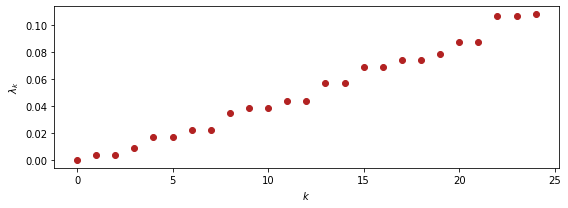
\includegraphics[width=0.5\textwidth]{Images/r2_eigenvals.png}
        \caption{Eigenvalues $\{\lambda_k\}, k=0, \dots, 24$}
    \end{subfigure}
    \hfill
    \begin{subfigure}[b]{\textwidth}
        \centering
        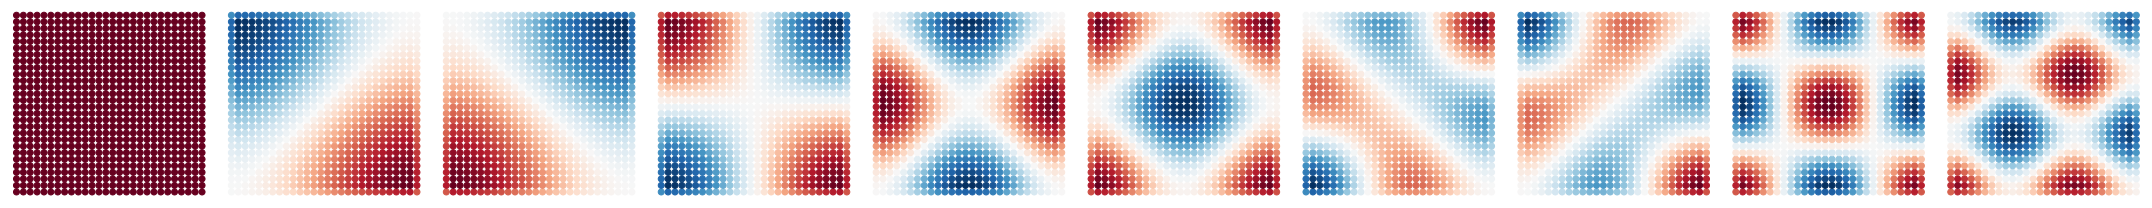
\includegraphics[width=\textwidth]{Images/r2_eigenvecs.png}
        \caption{$\{\phi_k\}, k \in \{0, 1, 2, 3, 4, 5\}$}
    \end{subfigure}
    \caption{Eigenvectors $\mathbb{R}^2$ manifold graph's eigenspace.}
    \label{fig:r2_eigenspace}
\end{figure*}

\begin{figure*}[h!] 
    \centering
    \begin{subfigure}[b]{0.9\textwidth}
        \centering
        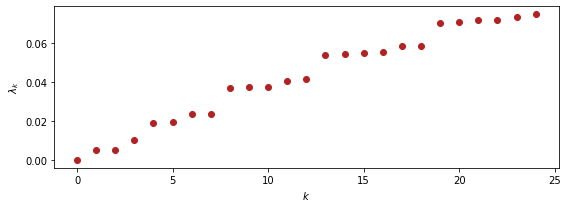
\includegraphics[width=0.5\textwidth]{Images/se2_eigenvals.png}
        \caption{Eigenvalues $\{\lambda_k\}, k=0, \dots, 24$}
    \end{subfigure}
    \hfill
    \begin{subfigure}[b]{\textwidth}
        \centering
        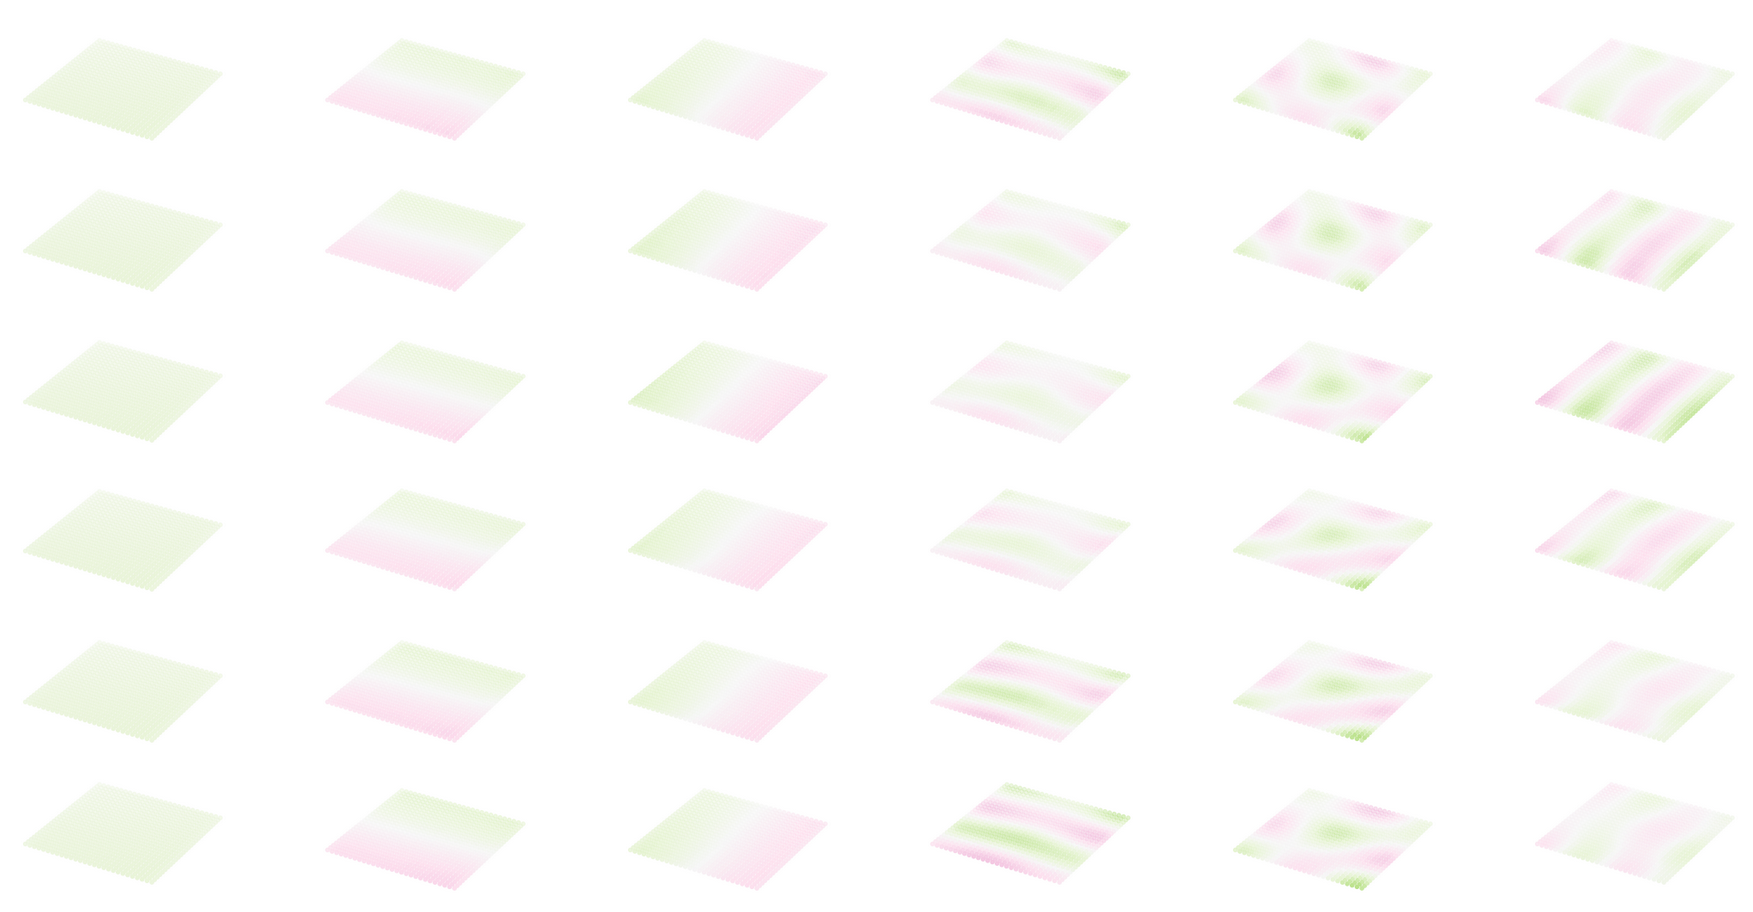
\includegraphics[width=\textwidth]{Images/se2_eigenvecs.png}
        \caption{Eigenvectors $\{\phi_k\}, k \in \{0, 1, 2, 8, 9, 10\}$}
    \end{subfigure}
    \caption{$SE(2)$ manifold graph's eigenspace. A column represents an entire graph, with six orientation layers stacked upon one other, from $\theta = -\pi/2$ (bottom) to $\theta = \pi/3$ (top).}
    \label{fig:se2_eigenspace}
\end{figure*}

\begin{figure*}[h!] 
    \centering
    \begin{subfigure}[b]{0.9\textwidth}
        \centering
        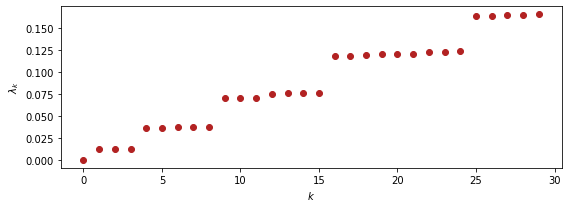
\includegraphics[width=0.5\textwidth]{Images/s2_eigenvals.png}
        \caption{Eigenvalues $\{\lambda_k\}, k=0, \dots, 29$}
    \end{subfigure}
    \hfill
    \begin{subfigure}[b]{\textwidth}
        \centering
        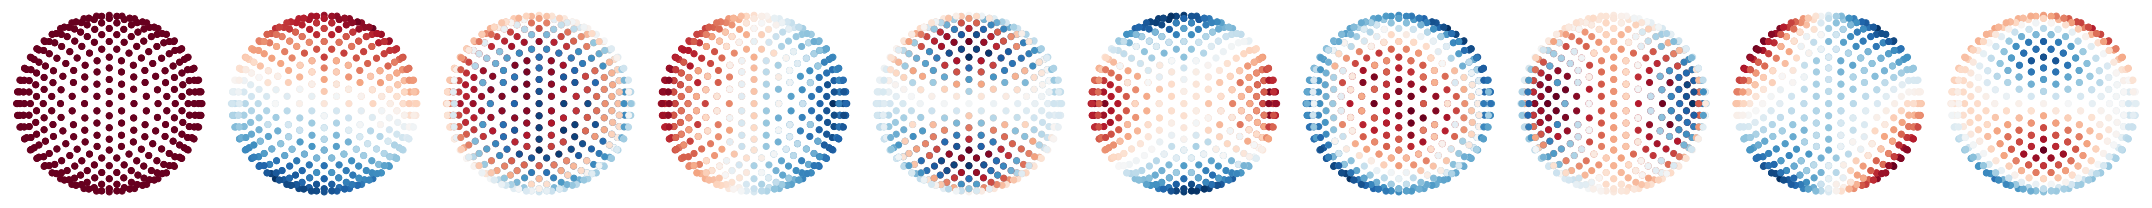
\includegraphics[width=0.8\textwidth]{Images/s2_eigenvecs.png}
        \caption{Eigenvectors $\{\phi_k\}, k \in \{0, 1, 2, 3, 4, 5\}$}
    \end{subfigure}
    \caption{$S^2$ manifold graph's eigenspace.}
    \label{fig:s2_eigenspace}
\end{figure*}

\begin{figure*}[h!] 
    \centering
    \begin{subfigure}[b]{0.9\textwidth}
        \centering
        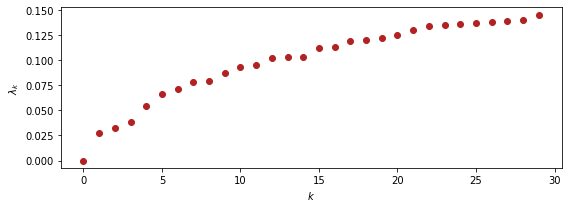
\includegraphics[width=0.5\textwidth]{Images/so3_eigenvals.png}
        \caption{Eigenvalues $\{\lambda_k\}, k=0, \dots, 29$}
    \end{subfigure}
    \hfill
    \begin{subfigure}[b]{\textwidth}
        \centering
        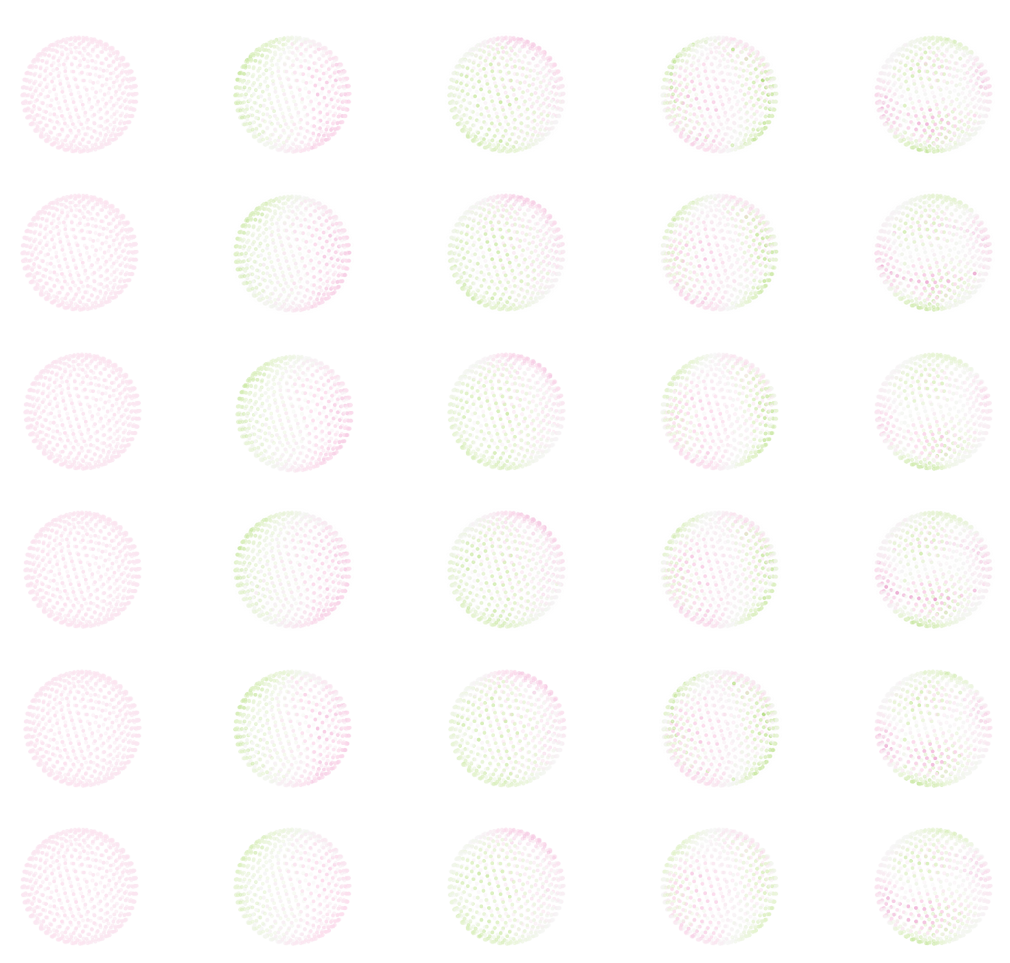
\includegraphics[width=0.8\textwidth]{Images/so3_eigenvecs.png}
        \caption{Eigenvectors $\{\phi_k\}, k \in \{0, 1, 2, 3, 4\}$}
    \end{subfigure}
    \caption{$SO(3)$ manifold graph's eigenspace. A column represents an entire graph, with six orientation layers stacked upon one other, from $\theta = -\pi/2$ (bottom) to $\theta = \pi/3$ (top).}
    \label{fig:so3_eigenspace}
\end{figure*}

\clearpage

\section{Equivariance leakage} \label{app:equivariance_leakage}

A powerful particularity of a group manifold graph neural network is that it is theoretically equivariant under any group transformation. However, further analysis of the test performances at each training's epochs suggests that our models are prone to an almost-equivariance leaking effect. It means that all along the training process, while the model is improving on the original test set, its performance on the flipped and rotated test set decreases (figure \ref{fig:equivariance_leaking}). This effect could be compared to an overfitting effect. 

\begin{figure*}[h!] 
    \centering
    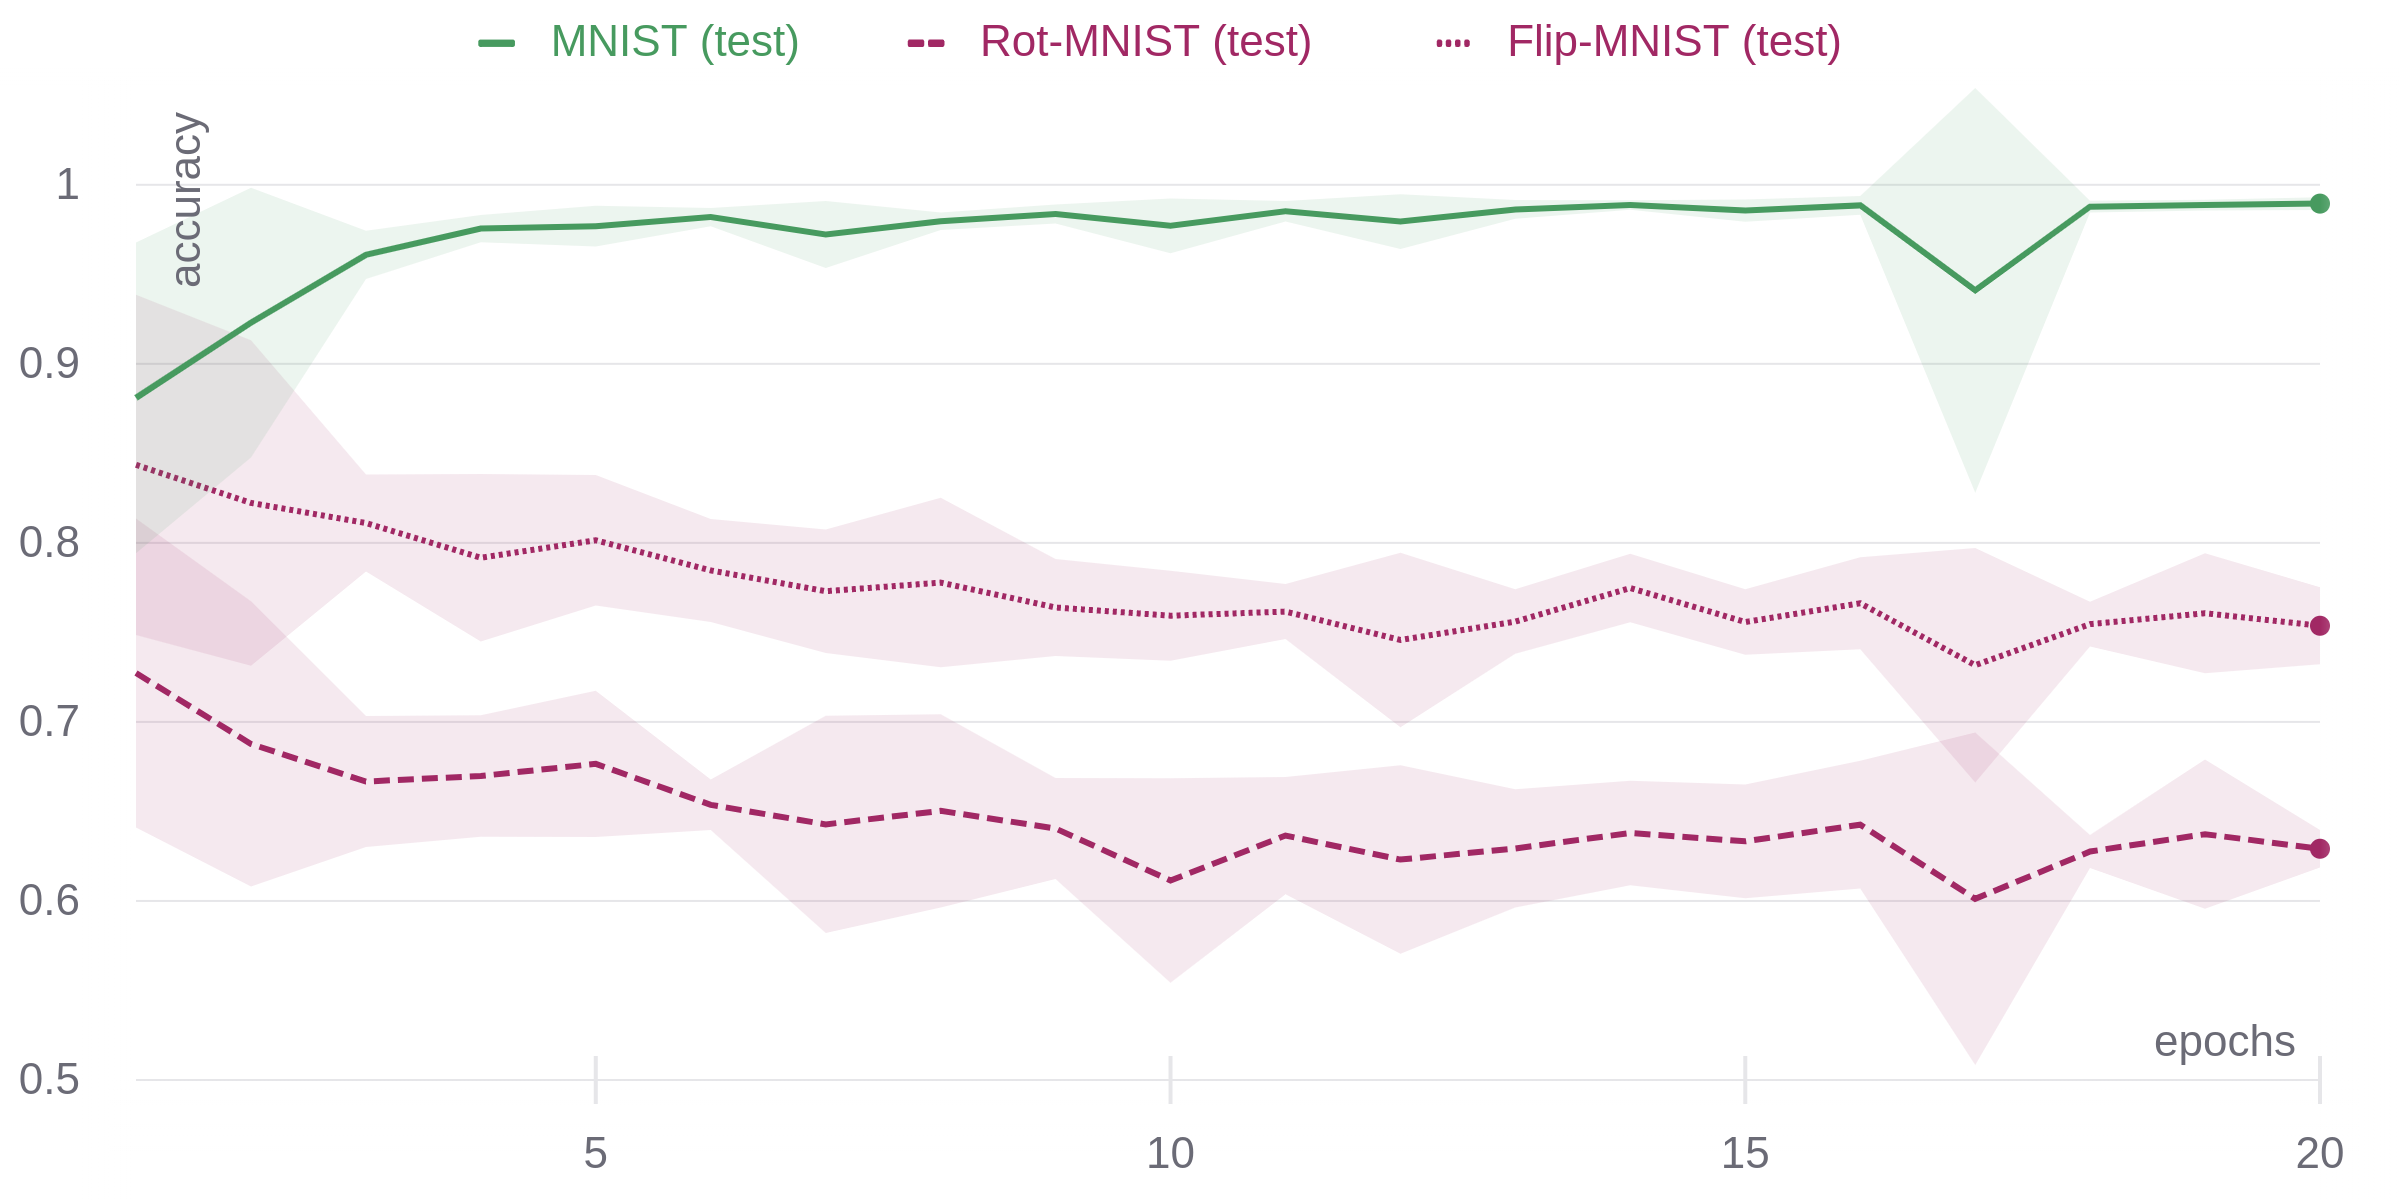
\includegraphics[width=10cm]{Images/equivariance_leakage.png}
    \caption{Mean of test accuracies on MNIST, Flip-MNIST and Rot-MNIST. Errorbars are 1 standard deviation computed over 10 trials.}
    \label{fig:equivariance_leaking}
\end{figure*}

We run experiments on MNIST, and models are evaluated on the three versions of the test set. There are two reasons for choosing MNIST to perform this experiment. First of all, this dataset is a trivial task, and any model could reach almost 99\% accuracy. It is also easy for a model to "overfit" on this dataset. If any over-fitting like effect should appear with our method, it would certainly appear on MNIST. The second reason is related to the complexity of the experiment. On MNIST, a model does not necessarily need to use pooling layers to perform exceptionally well. Because using pooling implies changing the graph data domain, it could be complicated to combine graph reduction with random perturbations on edges and nodes. We prefer to avoid such layers. We use $\xi = 0.0026$, $n_\theta = 6$, $\varepsilon = 0.1$ and Chebyshev kernel with size $4$. We analyze the effect of the sampling rate and the number of neighbors on the equivariance leaking and model performance. Because of its low resolution, MNIST is well-adapted to this kind of experiment since the effect of a too-low sampling rate will be observable very quickly, as we expect the majority of the pixels to be important.


For both methods, it is tricky to choose an optimal sampling rate and graph connectivity $K$. At a low sampling rate, the signal diffusion throughout the graph is very bad, and the model cannot perform well on any task. The required assumptions for the convergence of the graph Euclidean are not satisfied anymore (vertice sampling could lead to a far-from-uniform sampling of vertices while edge sampling makes the graph poorly connected). Naturally, the method does not help anymore to solve the equivariance leakage effect at a high sampling rate. The number of neighbors also plays an important role. Indeed, it makes the graph more robust to perturbations on edges and vertices, as more detour routes are available. Finally, these sampling methods help to reduce the computational complexity of the algorithm, as a small (vertices reduction) and sparse (edges reduction) graph Laplacian induced fast computations.

\begin{table}[h!]
\label{table:equivariance_leaking_results}
\centering 
\caption{Mean of test accuracies on three versions of the MNIST test set: original, flipped and rotated. Errorbars are 1 standard deviation computed over 5 trials.}
\begin{tabular}{c c c c c c c}
\toprule
& & & \multicolumn{4}{c}{MNIST} \\
$\kappa_{\mathcal{E}}$ & $\kappa_{\mathcal{V}}$ & $K$ & Test accuracy & F-Test accuracy & R-Test accuracy & Duration\\
\midrule
$0.50$ & $1.0$ & $8$ & $82.60 \pm 0.47 \%$ & $82.14 \pm 0.53 \%$ & $72.07 \pm 0.97 \%$ & $\sim \SI{3}{\hour}$ \\
$0.75$ & $1.0$ & $8$ & $95.23 \pm 1.68 \%$ & $93.15 \pm 2.67 \%$ & $81.89 \pm 3.87 \%$ & $\sim \SI{4}{\hour}$ \\
$0.90$ & $1.0$ & $8$ & $98.71 \pm 0.23 \%$ & $93.34 \pm 0.96 \%$ & $82.12 \pm 1.95 \%$ & $\sim \SI{4}{\hour}$ \\
$0.50$ & $1.0$ & $16$ & $95.09 \pm 0.50 \%$ & $94.97 \pm 0.53 \%$ & $88.59 \pm 1.00 \%$ & $\sim \SI{4}{\hour}$ \\
$0.75$ & $1.0$ & $16$ & $96.76 \pm 0.53 \%$ & $\boldsymbol{96.19 \pm 0.44 \%}$ & $\boldsymbol{88.19 \pm 0.18 \%}$ & $\sim \SI{5}{\hour}$ \\
$0.90$ & $1.0$ & $16$ & $98.62 \pm 0.18 \%$ & $95.16 \pm 0.73 \%$ & $87.37 \pm 1.31 \%$ & $\sim \SI{6}{\hour}$ \\
\midrule
$1.0$ & $0.50$ & $8$ & $89.04 \pm 1.18 \%$ & $88.83 \pm 1.17 \%$ & $83.81 \pm 2.34 \%$ & $\sim \SI{3}{\hour}$ \\
$1.0$ & $0.75$ & $8$ & $96.64 \pm 0.21 \%$ & $95.60 \pm 0.56 \%$ & $87.24 \pm 1.05 \%$ & $\sim \SI{4}{\hour}$ \\
$1.0$ & $0.90$ & $8$ & $97.24 \pm 0.45 \%$ & $92.54 \pm 1.55 \%$ & $80.43 \pm 1.20 \%$ & $\sim \SI{4}{\hour}$ \\
$1.0$ & $0.50$ & $16$ & $95.37 \pm 19 \%$ & $95.20 \pm 0.16 \%$ & $\boldsymbol{90.91 \pm 0.53 \%}$ & $\sim \SI{3}{\hour}$ \\
$1.0$ & $0.75$ & $16$ & $97.06 \pm 0.14 \%$ & $\boldsymbol{96.59 \pm 0.24 \%}$ & $90.48 \pm 1.19 \%$ & $\sim \SI{4}{\hour}$ \\
$1.0$ & $0.90$ & $16$ & $98.98 \pm 0.05 \%$ & $95.36 \pm 0.23 \%$ & $88.27 \pm 0.14 \%$ & $\sim \SI{5}{\hour}$ \\
\bottomrule
\end{tabular}
\end{table}

A natural question arises: do we better choose vertices or edges sampling? Well, it depends. According to the figure \ref{fig:sampling_results}, vertices sampling seems better if we want our model to be equivariant. Nevertheless, the convergence is slower than with edges' sampling, and the performance on the original test set is slightly less good. The only conclusion we can make is that, at least on MNIST, both methods work and reduce the equivariance leakage.

\begin{figure*}[h!] 
    \centering
    \begin{subfigure}[b]{\textwidth}
        \centering
        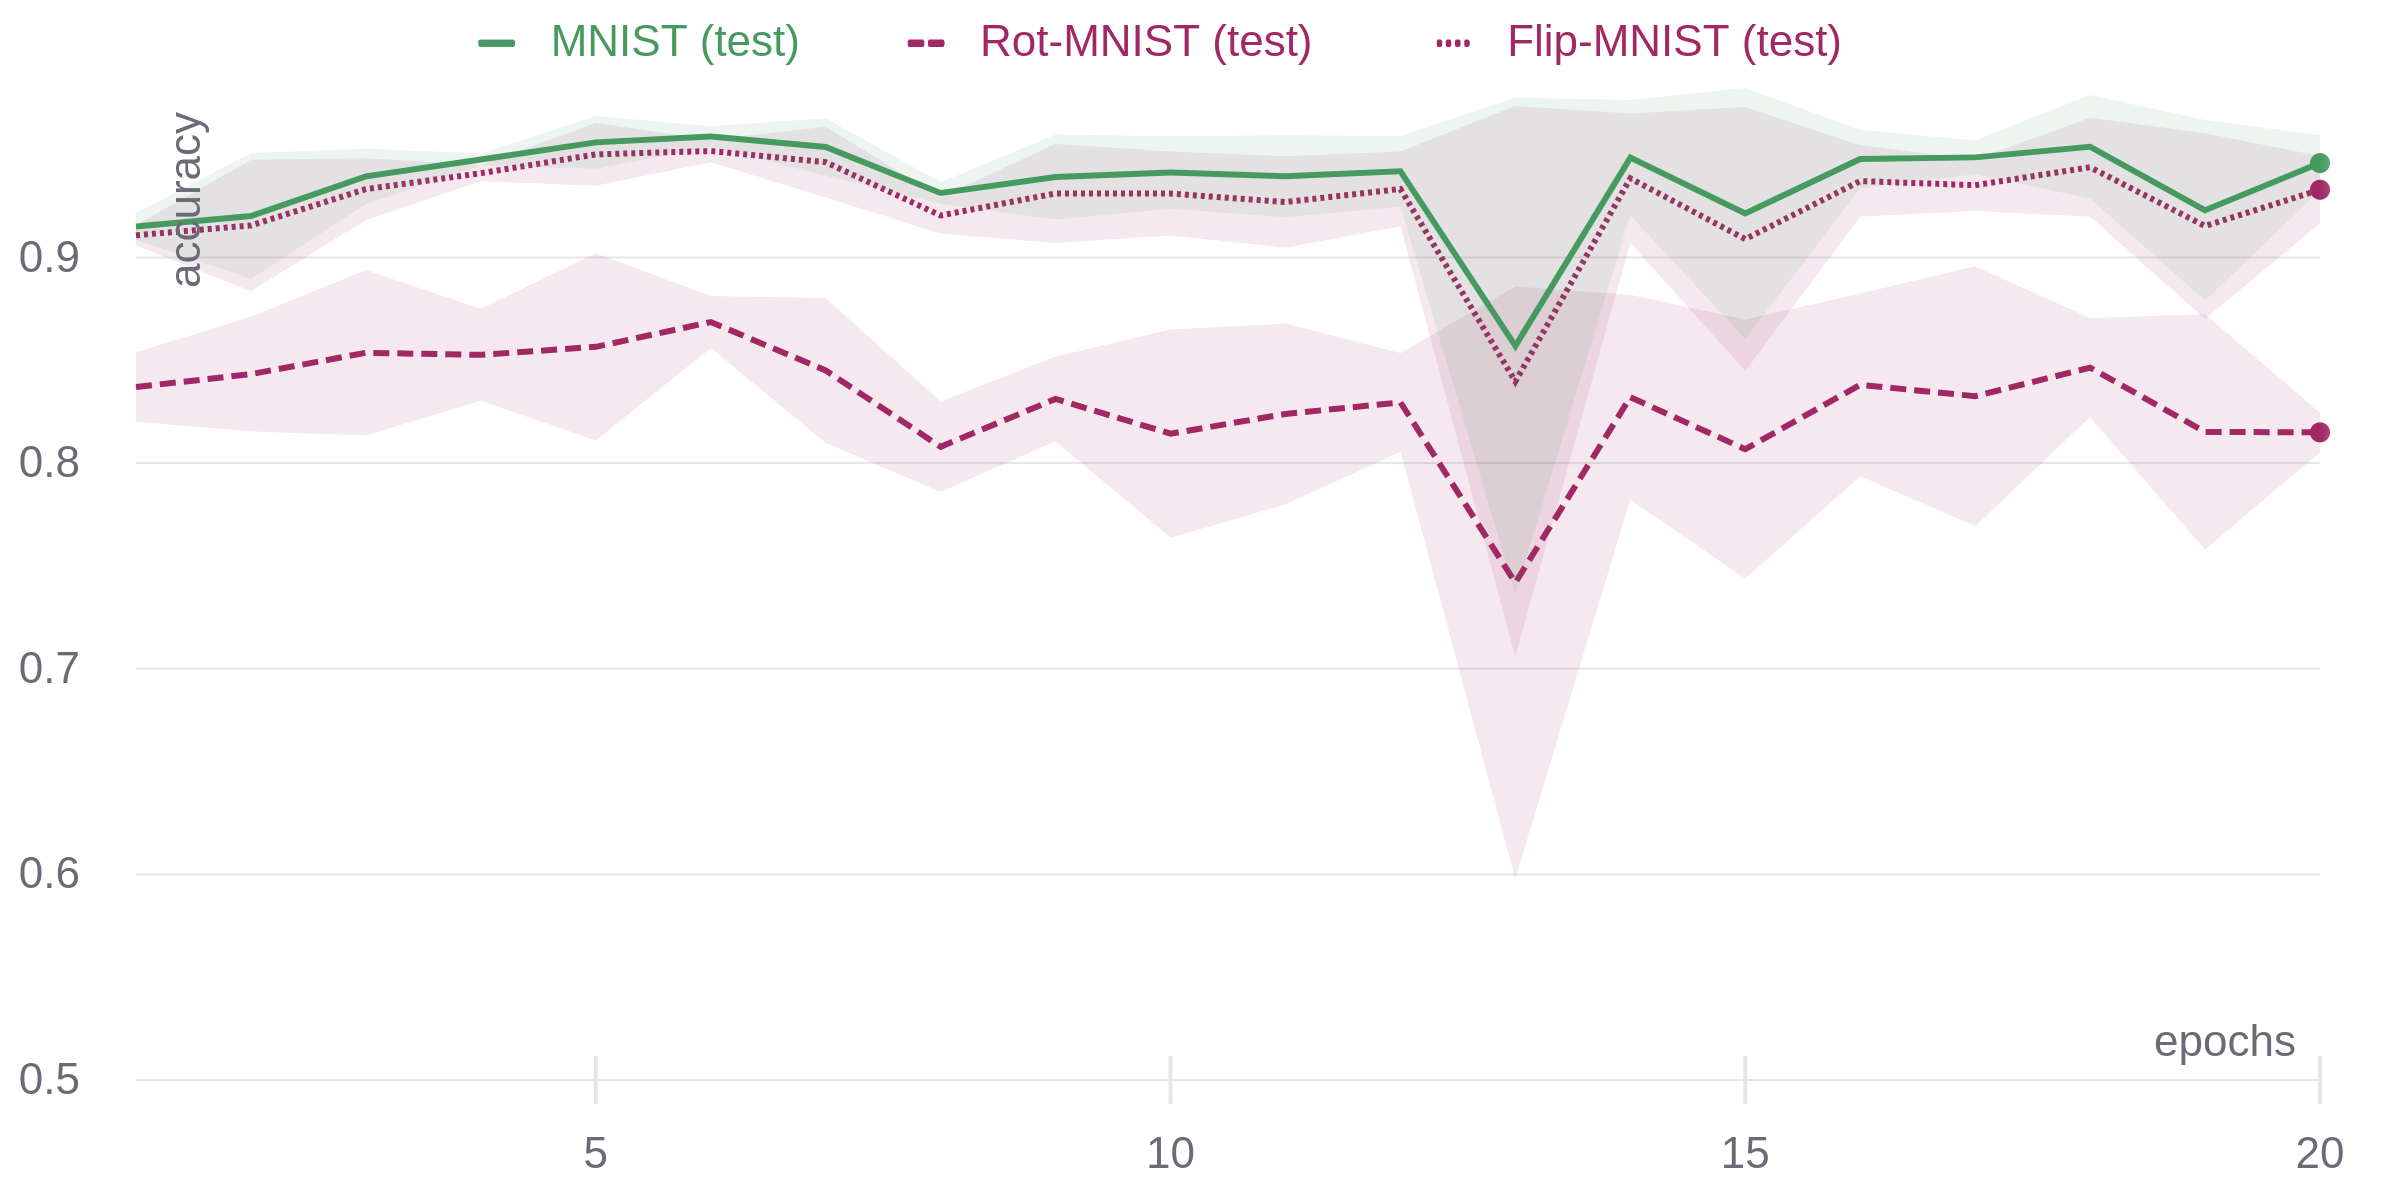
\includegraphics[width=0.8\textwidth]{Images/training_w_edge_sampling.png}
        \caption{Edges sampling with $K=16$ and $\kappa_{\mathcal{E}} = 0.75$}
    \end{subfigure}
    \hfill
    \begin{subfigure}[b]{\textwidth}
        \centering
        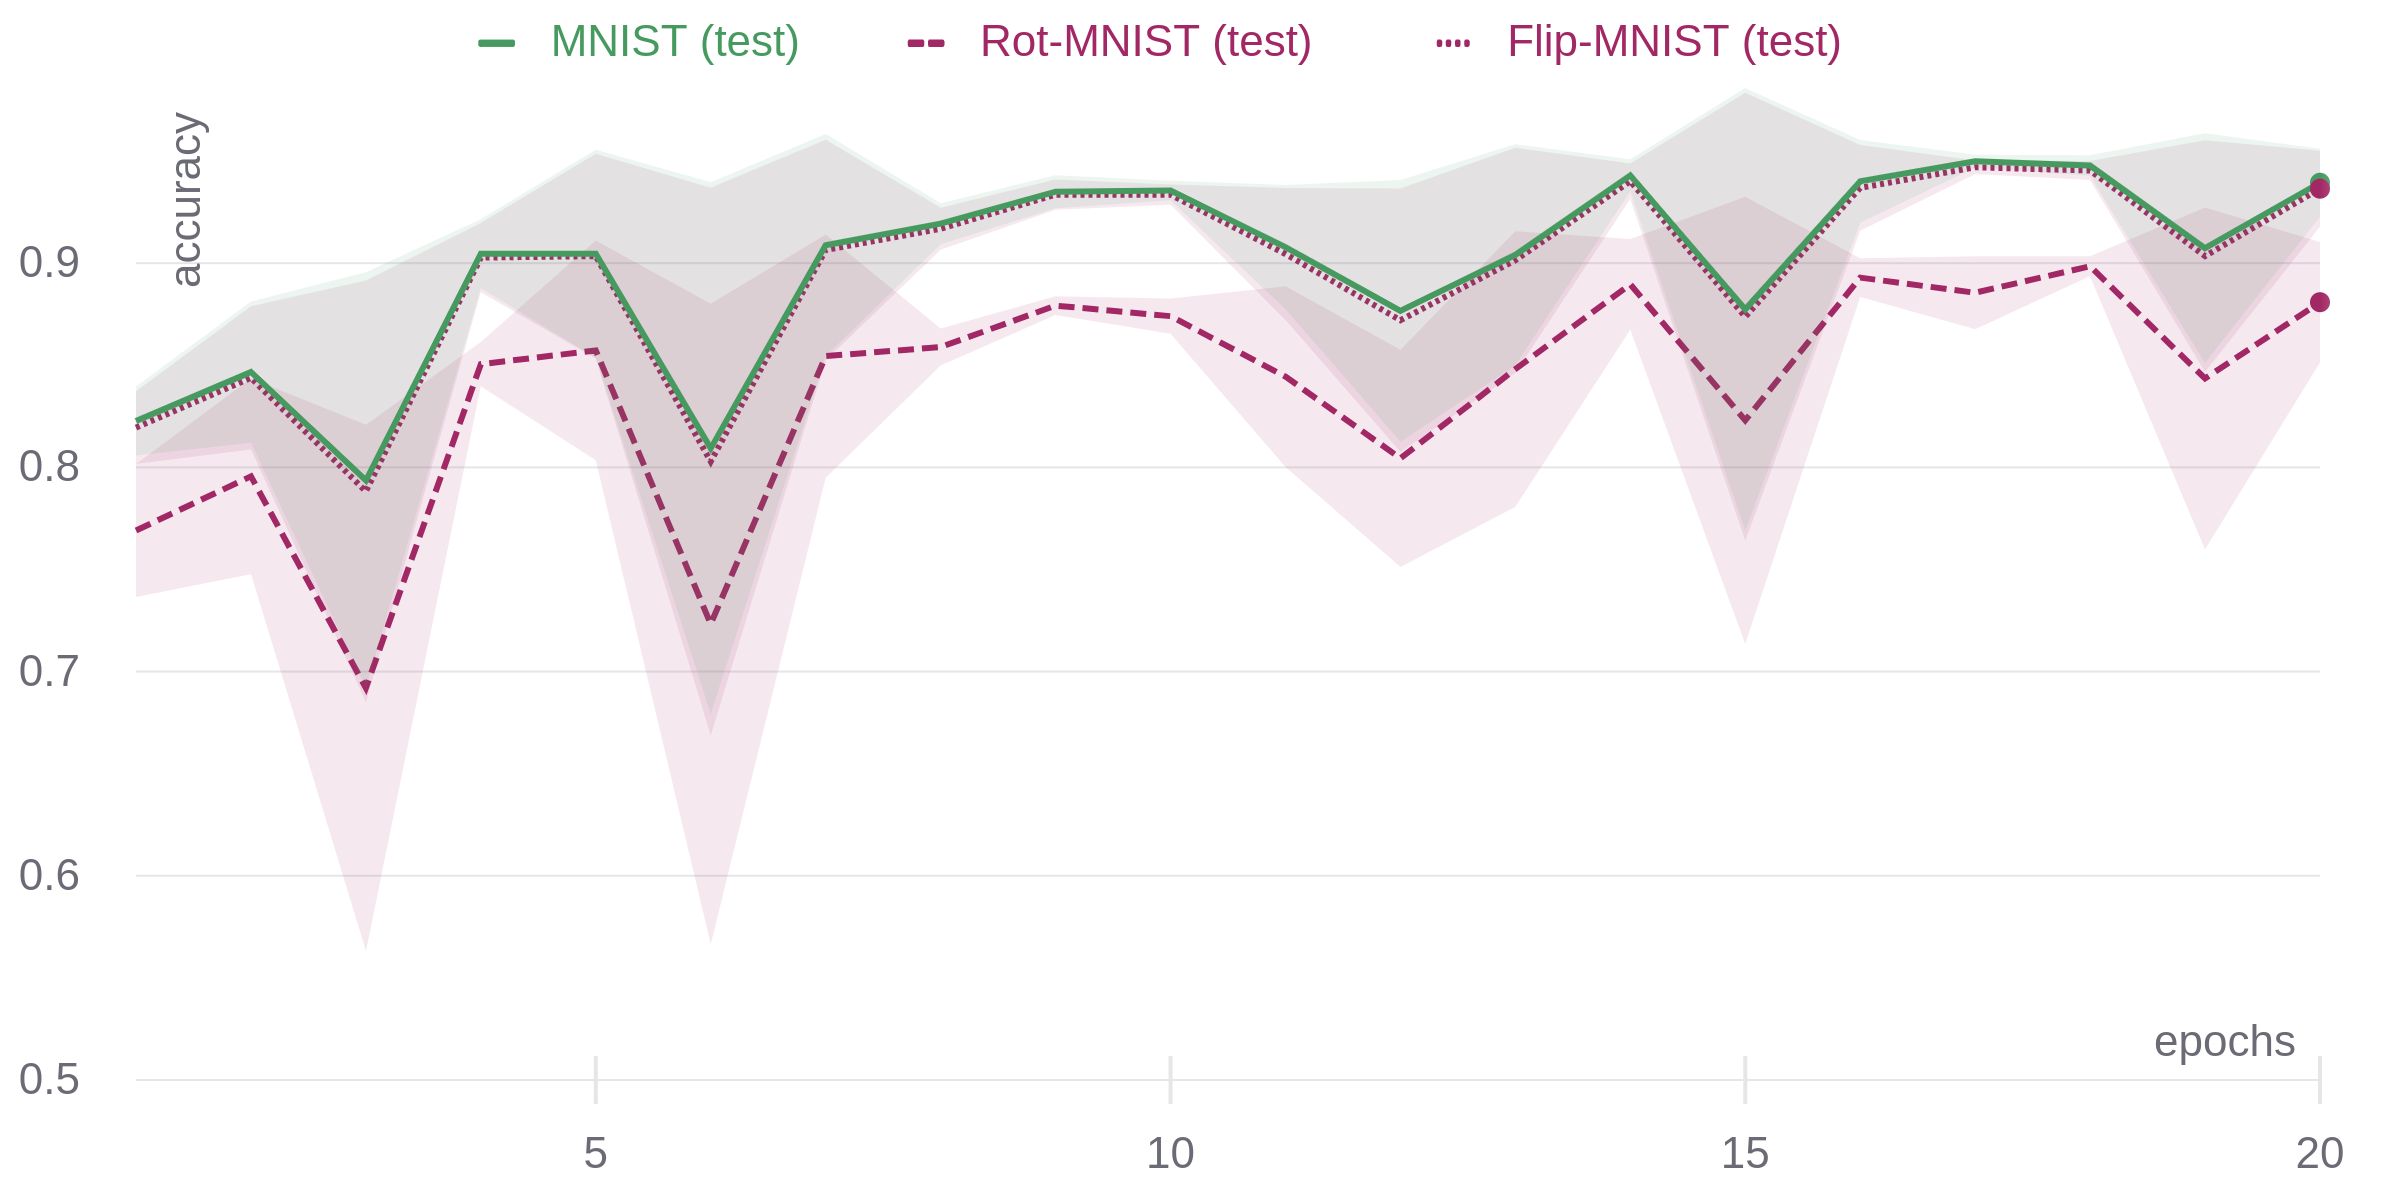
\includegraphics[width=0.8\textwidth]{Images/training_w_node_sampling.png}
        \caption{Vertices sampling with $K=16$ and $\kappa_{\mathcal{V}} = 0.75$}
    \end{subfigure}
    \caption{Mean of test accuracies on MNIST, Flip-MNIST and Rot-MNIST with edges and vertices samplings. Errorbars are 1 standard deviation computed over 3 trials.}
    \label{fig:sampling_results}
\end{figure*}


\end{document}
